\documentclass[]{msulabm}
\usepackage[utf8]{inputenc}
\usepackage{amsmath}
\usepackage{graphicx}
%\usepackage[linktocpage]{hyperref}  % if not using colorlinks, use linktocpage
\usepackage[colorlinks]{hyperref}  % if not using colorlinks, use linktocpage
\usepackage{bm}            % bold math
\usepackage{multirow}
\usepackage[table]{xcolor} % provide alternating rows with colors
\usepackage{textcomp}
\usepackage{xfrac} % gives split-level fractions with '\sfrac{a}{b}
\usepackage{multicol}
\usepackage[section]{placeins} % provides \FloatBarrier, to keep floats from crossing this barrier
\usepackage{amssymb}
\usepackage{wrapfig} % provides wrapping figures with text.
%\usepackage{enumitem} % gives \begin{enumerate}[resume] to resume counting from previous enumerate
%\usepackage{subfigure}
%\usepackage{tikz} % to draw arrows
\usepackage{xtab} % provides xtabular, tabular environment that spans multiple pages and other awesome things
\usepackage[style=phys,biblabel=brackets,pageranges=false]{biblatex}
\usepackage{pdflscape}
\usepackage{ragged2e}
\usepackage{longtable}
\usepackage{mathabx} % gives astronomy symbols like \Earth
\usepackage{pdfpages}

\bibliography{references-manual,bbarker-zotero}

\newcommand{\abs}[1]{\left\lvert#1\right\rvert}

\title{Laboratory Manual}
\author{PHSC 12710 Galaxies \\ \\ The University of Chicago}
\date{Winter 2021}

\pagestyle{ruled}

\definecolor{lgray}{rgb}{.2,.2,.2}

\makeevenfoot{ruled}{\thepage}{\footnotesize{\textit{Last updated \today}}}{}
%\makeevenfoot{ruled}{\thepage}{}}{}
\makeoddfoot{ruled}{}{\color{lgray} \tiny{This work is licensed under \href{http://creativecommons.org/licenses/by-sa/4.0/}{CC BY-SA 4.0} by \href{mailto:bbarker@uchicago.edu}{the University of Chicago}.}}{\thepage}


% allows us to use subcaptions from the memoir class in figures. See Memoir Section 10.9
\newsubfloat{figure}

% don't worry so much about filling every page.
%\raggedbottom

% raise the penalty for splitting footnotes across different pages. Default is 100.
\interfootnotelinepenalty=10000

%\includeonly{amplifier/amplifier} 

% creates a standard length to use 
\newlength{\answerskip}
%\setlength{\answerskip}{90pt} 

%% use plus / minus if latex is squeezing the answer space too much
\setlength{\answerskip}{2cm plus 0.2cm minus 0.2cm}

\newlength{\qaskip}
\setlength{\qaskip}{\answerskip}
\addtolength{\qaskip}{\baselineskip}

% reduce vertical space between chapters in table of contents. Default is 2em.
\setlength{\cftbeforechapterskip}{1em}

% allow for extra line on a page to help prevent widow/orphan lines.
\sloppybottom

% Now we can caption a table outside of the table float environment (good for multi-page tables)
\newfixedcaption{\freetabcaption}{table}

%\includeonly{snells-law/snells-law}
%\includeonly{ohms-law/ohms-law}

\begin{document}
\maxtocdepth{chapter}

 % start roman numbering
 \frontmatter

\maketitle

%\clearpage

%Brent W. Barker

%Department of Astronomy \& Astrophysics

%The University of Chicago

%5640 South Ellis Ave.

%Chicago, IL 60637

%\href{mailto:bbarker@uchicago.edu}{bbarker@uchicago.edu}

%\vspace{2\baselineskip}

%\includegraphics{cc-by-sa-88x31}

%\textcopyright{} 2018 Brent W. Barker. Except where otherwise noted, this work is copyrighted under the Creative Commons Attribution-ShareAlike International 4.0 License. To view a copy of this license, visit \url{http://creativecommons.org/licenses/by-sa/4.0/}.

%\vspace{\baselineskip}

%These labs, excluding "Impulse and Momentum" and the appendices, are a derivative of "\href{https://%sites.google.com/site/scientificabilities/ISLE-labs}{ISLE Labs}" by the Rutgers Physics and Astronomy %Education Research group, used under the Creative Commons Attribution International 4.0 License.
%To view a copy of this license, visit \url{http://creativecommons.org/licenses/by/4.0/}.

%At Rutgers University, many people contributed to this project over the years.
%The list of names is very long and includes: Eugenia Etkina, Alan Van Heuvelen, Suzanne Brahmia, David %Brookes, Michael Gentile, Anna Karelina, Michael Lawrence, Marina Milner-Bolotin, Sahana Murthy, Maria %Ruibal-Villasenor, Aaron Warren, Xueli Zou.

 % skip to next right leaf (``recto'')
 \cleartorecto

 % the star means that the ToC itself is not listed in the ToC
 \tableofcontents*

 % start arabic numbering
\mainmatter 


%\chapter{Observing with small optical telescopes}

In this lab, we will be using a reflecting optical telescope to observe objects in the KPTC
lab. This will give you practice using the CCD camera to take images. More importantly,
these activities aim to give you a sense of scale for what the combined telescope and CCD are
capable of, and why this is useful for astronomical observations. The goal is for you to build some
understanding and appreciation for how telecopes of this size, equipped with a digitial camera and
filters, can be used to take images, and how those images relate to the capabilities of your most
familiar imaging system --- i.e. your eye.
%Your project work with the Stone Edge Observatory use a similar (although somewhat larger telescope) setup; this lab is designed to let you
%get your hands on the hardware and build some understanding for how it works and what it can
%do.

%\textbf{Rubric Rows to be assessed:} B5, B9, D2, D4. These are referenced in the lab manual where they should be addressed.

\section{Reflection Telescopes}

The primary utility of a telescope is its ability to gather light, thereby enabling visualization and analysis of the faint astronomical objects we are trying to observe. This requires focusing light incident on a large surface area. We will be using a \textbf{reflecting} telescope, which means that light rays from observation targets are focused into an eyepiece or onto a detector with reflecting mirrors. This is in contrast to refracting telescopes, which use refracting lenses to focus light rays. Figure~\ref{sot:fig:schmidt} shows schematically how this kind of telescope works. 

\begin{figure}
	\centering
	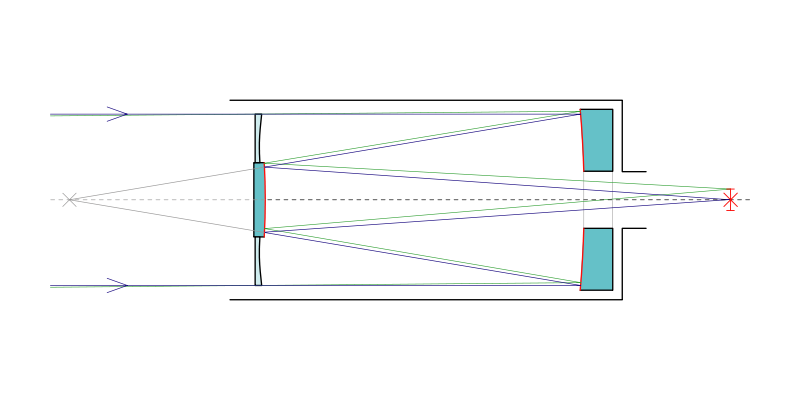
\includegraphics[scale = 0.5]{small-optical-telescopes/Schmidt-Cassegrain-Telescope.png}
	\caption{Schematic for a reflecting telescope of a Schmidt-Cassegrain design. 
		Light rays from astronomical objects enter the telescope in parallel because their source is effectively at infinity. They are then reflected by a parabolic primary mirror onto a secondary mirror that again reflects the light to a focus. An eyepiece or a camera is placed at the focal plane of the resulting image. Image source: \url{https://en.wikipedia.org/wiki/Cassegrain\_reflector\#/media/File:Schmidt-Cassegrain-Telescope.svg}}\label{sot:fig:schmidt}
\end{figure}

To take images in this lab,
% and to observe astronomical objects using the SEO,
 we make use of a \textbf{Charge Coupled Device (CCD)}. CCDs are the standard detectors for taking astronomical images at wavelengths blueward of approximately 1 micron. Think of the CCD we are using as a
very advanced low-noise digital detector, not wholly dissimilar from the digital detector in your
smartphone. Every time a photon within a certain energy range hits the detector, an electron is knocked off of the incident pixel, charging that pixel's capacitor. Thus, for each pixel, more photons $\implies$ more electrons $\implies$ more charge, and the charge can be read off into a digital signal that is then processed as an image. 

The main thing to note is that the CCD material is not sensitive to all wavelengths of light uniformly. Photons of certain energies are more likely to excite electrons in the detector and thus contribute to the output image. Consequently, the observed image intensity will be weighted by the response function of the detector.

\subsection{Filters}
Light is composed of photons with energies that determine their wavelengths (sorter wavelength $\implies$ higher energy). Thus every light source exhibits a textbf{spectrum} of energies based on its energetic components, determined by the physics of the light emission process. Thus, observing the energetic constituents of light from astronomical objects - a.k.a. observing the spectrum of emitted radiation - is a fundamental tool in observational astrophysics. However, obtaining the specific intensity of radiation as a function of energy from an astronomical source is challenging. An easier way to asses the electromagnetic energies observed is to image them in different filters: materials that are transparent to a known range of wavelengths and opaque to all others. Thus, one can image the same object with multiple different filters to get a sense of the wavelength regimes that make the strongest contributions to the overall electromagnetic output. 

A filter is characterized by its \textbf{transmission function}: a function that characterizes the amount of light that is transmitted by the filter at each wavelength. Figure~\ref{sot:fig:filters} shows the transmission functions for some standard astronomical filters (similar to the ones you'll be using in this class).

\begin{figure}
	\centering
	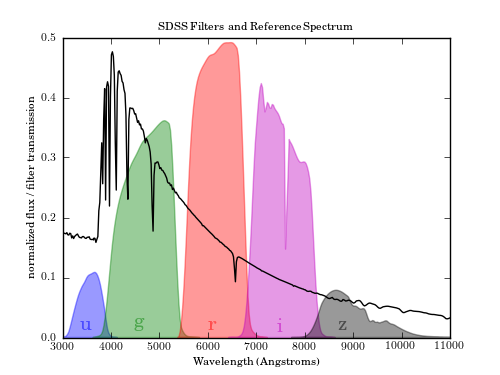
\includegraphics{small-optical-telescopes/fig_sdss_filters_1.png}
	\caption{Filter Transmission Functions for the Sloan Digital Sky Survey, overlaid on a stellar spectrum (in this case the spectrum is probably an
		A-type star). The magnitude observed by each filter will be proportional to the integrated spectrum multiplied by the filter transmission. It's clear in this image that the underlying spectrum of the star will cause the different filters to have different magnitudes. How would these magnitudes change if the spectrum was, say, of an M-star instead? (Image source: \url{http://www.astroml.org/\_images/fig\_sdss\_filters\_1.png})}\label{sot:fig:filters}
\end{figure}

\section{Lab Tasks: Introduction}

The telescope and camera assembly is an expensive and relatively fragile piece of hardware, so
move carefully when interacting with the system. We have only one setup, and there are
three main observing tasks, so before starting divide into three groups. Each group
will set up and control the telescope and camera for observing in one of the sections below, assisted by others in the lab, and
then share the output images with everyone in the lab group.

\section{Telescope Set Up, Preliminary ``Observations"}\label{sot:sec:setup}

First we will be observing an object at the opposite end of the lab room with the lights turned off. During this exercise we will 1) check that the telescope is focused (which should already be the case), 2) gain practice positioning the telescope and targets, and 3) demonstrate the light gathering and angular resolution capabilities of the telescope with a physical object for which you have an direct sense of scale. \textbf{NOTE: For safety purposes, do not walk around the
	lab while the lights are off; instead, turn the lights off only as needed to gather data
	or make observations, and when the lights are off, don’t move about significantly.}

\begin{steps}
	\item The telescope should already be set up, with the camera on and cooled, and be approximately
	in focus and pointed at the target at the other end of the lab bench. If not, your TA will
	work with you to get the setup roughly correct.
	
	\item Your first task will be to tweak the centering of the image target. This doesn't have to be
	perfect, but you should be able to see the mm scale marks. The telescope can be moved in elevation (up-down). The fine control of elevation is achieved using a knob on the mount - your TA will show you details. To shift the image left or right, move the target instead.
	
	\item Next we want to precisely focus the telescope. Do this with most of the lights off - otherwise
	the image has too much light. Use the 4th filter of the five available; this can be selected
	from the ‘Filter’ menu. Then, use the \textbf{Focus} task from the camera control system toolbar,
	and take images of a few seconds (at most). If the image is completely dark, and the peak intensity number in the focus box is reading around 65000, then the CCD is saturated, and the light in the room should be reduced, or the exposure time shortened.
	
	\item Start the focus sequence - the camera will just
	take and display images repeatedly, of the exposure duration you specified. Now, adjust
	the focus knob (on the back of the telescope, off center) until you achieve an optimal focus.
	Note that you can (and should) zoom the magnification of the image so you can see the
	imaging target in detail. Do this by adjusting the magnification, and adjusting the image
	x,y centering so you’re looking at an appropriate zoomed location in the image. Note that
	you’ll need to not be touching the telescope or mount to get a sharp image, so you’ll
	have to adjust, then move away, wait, and repeat. Your classmates walking around the lab
	will cause image shake that will make focusing difficult, so enforce a still classroom while
	you do this.
	
	\item Time to demonstrate one helpful aspect of telescopes by taking an image in the dark. Once the telescope is focused to the sharpest possible images, turn off the lights and acquire an image using the
	\textbf{Grab} button on the toolbar. An exposure time of 40--60 seconds is usually good with all of
	the lab lights off and the blinds closed.
	
	\item Save this image in ‘fits’ format; the ‘ds9’ tool available on all of the lab
	computers can be used to examine the image in detail.
%	We’ll use the university supported ’Box’ system to share data with your lab classmates.
%	See \url{uchicago.account.box.com/login} for details.
	
	\item With the lights back on, gather around the target on the lab bench and then
	turn the light off again. Observe the target. Can you see it? Can you see the details? Does
	it matter how close you are?% (Rubric Row B5)?
	
	\item Compute and report the ratio of the light gathering power of
	the telescope relative to your eye, and comment on how that relates to what you do (or do
	not) observe by eye compared to the telescope.% (Rubric Row B9).
	
	\item In the acquired and saved image you can see a mm scale, which correponds to some number
	of pixels. Compute and report the ‘plate scale’ in mm/pixel. Given the distance between the
	telescope and the target, what is the angular plate scale in arcseconds/pixel?
	
	To find this, note that for an arc (segment) of a circle, the length of that arc $s$ is related to the radius of circle $r$, and the angle (in radians) subtended by that arc $\theta$ by
	\begin{equation}
	 s = r \theta
	\end{equation}
	
	\item What do you
	think is the smallest feature (in arcsec) that you could resolve using this setup? Would we
	expect to see images of stars that sharp if we turned the telescope and camera skyward?
	Also, what is the field of view (arcseconds $\times$
	arcseconds) of this camera+telescope setup? Finally, observe the target from the vantage
	point of the telescope by eye. What detail can you see? How does that compare to what
	you can see with the telescope?
\end{steps}

\section{Grating Spectrum and Filters}\label{sot:sec:grating}

The next portion of the lab will involve observing a grating spectrum projected onto a blank white
target. We will use this to understand how the filters work. In addition, you will combine the
outputs of this and the third portion of the lab to unambiguously identify the 5 filters in the filter
wheel.
\begin{steps}
	\item Replace the reticle target and box with the blank white target mounted in a stand. Ensure
	the stand is placed so the target occupies the same plane as the reticle target did (otherwise,
	you’ll need to refocus the telescope; The paper has a pen mark on it - use this a reference if you do need to tweak the focus.). Next, place the light box with the attached diffraction
	grating on the same wooden stand using in the previous section, pointed toward the white target, and plug the light box in.
	This should generate a rainbow on the target screen. You may need to turn the lab lights
	off to see the rainbow easily. This rainbow is the spectrum of the incandescent lamp inside
	the light box.
	
	\item Once you’ve configured the setup, turn the lab lights off, and grab an exposure of 1 second
	in the 4th filter (if this section follows the above, that filter should already be selected).
	The bright band in the image should be positioned in the center of the image. If not, adjust
	the position of the spectrum by rotating the stand holding the lightbox+grating around the
	vertical axis to move spectrum slightly left or right on the screen. Adjust until the light band of the image is centered left/right. Also,
	to center vertically so that the light fully covers the image along the vertical axis, you may
 adjust the telescope elevation. To do these adjustments, you may find it easiest to put the camera
	in focus mode again. Centering vertically is less important - so long as a significant portion
	of the image contains light on the vertical axis there is no particular need to fine-tune the
	vertical alignment.
	
	\item Once you have the telescope aligned and focused on the reflected grating spectrum, grab an
	image of 1 second for each filter available in the CCD filter wheel. Save each image and note
	the differences. Comparing the different images, where are the bands located? How constant is the intensity of
	light across the band in the horizontal direction? How broad/narrow are the bands? What
	is the physical explanation for these observations (see also the end of the next section)?
\end{steps}

\section{Indirect H-lamp observations}\label{sot:sec:h-lamp}

\begin{steps}
	\item Now we will make some observations to demonstrate the utility of the narrow-band filters.
	Turn off the lamp with the grating attached and remove it from the lab bench. Remove the
	white screen that was used to reflect the grating spectrum, and again place the reticle target
	on the box (same as the activities for Section~\ref{sot:sec:setup}) at that location and refocus on the target if necessary.
	
	\item If the Hydrogen lamp is not already in place and set up, place the Hydrogen lamp in front
	off to side, plug the tube of Hydrogen gas into the lamp stand, and plug this
	into an electrical outlet. Use the pedal to turn it on and make sure it’s working: it will be
	a bright and somewhat odd (to your eye) magenta color (why?). Also, have a look at the
	Hydrogen lamp by eye, using the unmounted gratings --- note what you see, and explain what you
	see in your lab report. How many emission lines are visible?
	
	\item Make sure the reticle target is in the field of view of the telescope, similar to Part 1. Turn
	off the lab room lights, leave the Hydrogen lamp off, and grab a 10 second image in each of
	the 5 filters. Save each image as a fits file, with a name that indicates the filter and lamp
	condition (for example ’\texttt{filter1nolight.fits}’ etc.) The image should be dark but the target should
	be visible at least in some cases. Now, turn on the Hydrogen lamp using the small attached
	pedal, and grab another set of images (one per filter, ten seconds in each case) and similarly
	save them. You may find it easier to take each filter sequentially, turning the lamp on and
	off, rather than doing all filters lamp off and then lamp on. Do what works best for you.
	
	\item One of the two narrowband filters in the wheel - see Figure~\ref{sot:fig:filters} to know
	which filters are narrow in wavelength - is an H-alpha filter that isolates emission at the
	wavelength of the H-alpha Balmer line. Which filter is this? Filter1? Filter2? Filter3?
	Explain, using the data taken.
\end{steps}

The filter wheel contains two narrow band and three broad band filters. As already indicated
above, one of the narrow band filters is H-alpha, and the other is OIII-5007 (an emission line
at 500.7nm from star forming regions that is strong in star-forming galaxies, such as the Milky
Way). The broad band filters are the g-band (’g’=green) r-band (’r’=red) i-band (’i’=infrared) ;
see Figure 2 for details.

\begin{steps}
	
	\item Based on the data taken in Sections~\ref{sot:sec:grating} and \ref{sot:sec:h-lamp}, deduce the identification of each filter; provide your final list in your lab report - i.e. filter 1 as ’this’, filter 2 is ’that’ etc. Describe step-by-step how you solved this problem.
% (Rubric Rows D2, D4 (do not worry about experimental uncertainties, since this is a qualitative problem)).
\end{steps}

\section{Optional Section: See yourself with a telescope!}

Time permitting, you can also take images of yourself with the telescope.
Try placing your hand where the imaging target are (use the wooden box a
rest stand). Take images at different wavelengths (if you stayed carefully
still, you could make a color composite), or even see what your fingers
look like in H-alpha light). Or, place a stool nearby, take a seat, and
snap a partial portrait. Your face is far too large to fit in the field of
view at that distance, but your eye would fit! (refocusing will be
necessary in this case...)

\section{Report checklist and grading}

Each item below is worth 10 points, and there is an additional 10 points for attendance and participation. See Appendix\ \ref{cha:lab-report-format} for guidance on writing the report and formatting tables and graphs.

\begin{itemize}
	
	\item Image of the target that you captured and qualitative observations (Steps 6--7)
	
	\item Ratio of light-gathering power (Step 8) with comments.
	
	\item Calculation of pixel scale, questions regarding resolution and field of view. (Steps 9--10)
	
	\item Images of spectrum with each filter with analysis (Step 13).
	
	\item Qualitative observations of the hydrogen emission with diffraction gratings (Step 15).
	
	\item Images of hydrogen emission with each filter and identification of H-alpha filter (Steps 16--17).
	
	\item Identification of each filter in the filter wheel, with justification (Step 18).
	
\end{itemize}
\chapter{Measuring distant objects with parallax}

%todo make two more telescopes on tripods, to have two setups going at a time. each group can use one telescope at a time, as long as scopes don't move.

%todo difference between measurement uncertainty and comparing between known and unknown quantities.


\section{Introduction}

Since it takes time for light to travel to us from objects in the universe, the further out an object is, the further back in time we see it. So for us to have an accurate picture of how the universe was in the past, we need to know how far away things are. For things that are nearby on Earth, we can travel there and see how far we went, or how long we took to get there. For things further away like the moon, we can use Kepler's laws, or we can bounce a beam of light off of it and see how long it takes to get back. For objects outside of our solar system, it would take too long, and the light would disperse too much, for us to use this last technique. For those objects that are still relatively nearby, we can use the parallax technique as the first rung on our distance ladder.

\section{Forming Groups}

If you are attending the lab session live and do not yet have a group, one way the TA could assist is to arrange "speed networking" among those who still need a group. This would involve the TA organizing Zoom Breakout Rooms, where each room is 2-3 students, and each group talks about how they work and what they are looking for in a group member. Then after 5 minutes or so, the Rooms are changed so people are with different people. This could help people get to know each other enough to form lab groups.

\begin{steps}
	\item Once you have a group, meet with each other and decide a) what tools you will use to communicate and collaborate, b) when you will meet, c) what you will do when you need to change an agreement, and d) what you will do when you a person has an issue with how the group is functioning.
%\textbf{Write this in your lab report. This part counts as data collection and analysis, so it can be identical in each member's report.}
\end{steps}

\section{Team roles}

\textbf{Decide on roles} for each group member. The available roles are:

\begin{itemize}
	\item Facilitator: ensures time and group focus are efficiently used
	\item Scribe: ensures work is recorded
	\item Technician: oversees apparatus assembly, usage
	\item Skeptic: ensures group is questioning itself
\end{itemize}

These roles can rotate each lab, and you will report at the end of the lab report on how it went for each role. If you have fewer than 4 people in your group, then some members will be holding more than one role. For example, you could have the skeptic double with another role. Consider taking on a role you are less comfortable with, to gain experience and more comfort in that role.

Additionally, if you are finding the lab roles more restrictive than helpful, you can decide to co-hold some or all roles, or think of them more like functions that every team needs to carry out, and then reflecting on how the team executed each function.

\section{Installing SAOImage DS9}

SAOImage DS9, or DS9 for short, is an image viewer, analyzer, and processor written and used by astronomers for working with astronomical images.

\begin{steps}
	\item Download and install DS9 from \url{http://ds9.si.edu/site/Download.html}. SAOImage DS9, or DS9 for short, is an image viewer, analyzer, and processor written and used by astronomers for working with astronomical images.
	
	If you click the link to download, it might say "redirecting" while never actually redirecting. In this case, copy the link into the address bar directly.
	\begin{framed}	
		\textbf{For MacOS}, unless you know otherwise, choose from the top set of choices (to the right of
		the blue apple logo). To find your version, from the Apple menu in the corner of the screen,
		choose “About This Mac”.
		
		If it displays a warning and prevents you from installed from an unidentified developer, follow the instructions at the following link to create an exception:
		
		\url{https://support.apple.com/guide/mac-help/open-a-mac-app-from-an-unidentified-developer-mh40616/mac}
	\end{framed}
\end{steps}

\section{Worksheet}

Complete the worksheet ``The Parsec'' on the following pages. You can draw the diagrams needed and include a picture of your diagrams, or use a drawing program to draw on them.
%Each member of the group will turn in their own worksheet as part of their lab report, and you can work in groups to complete them.

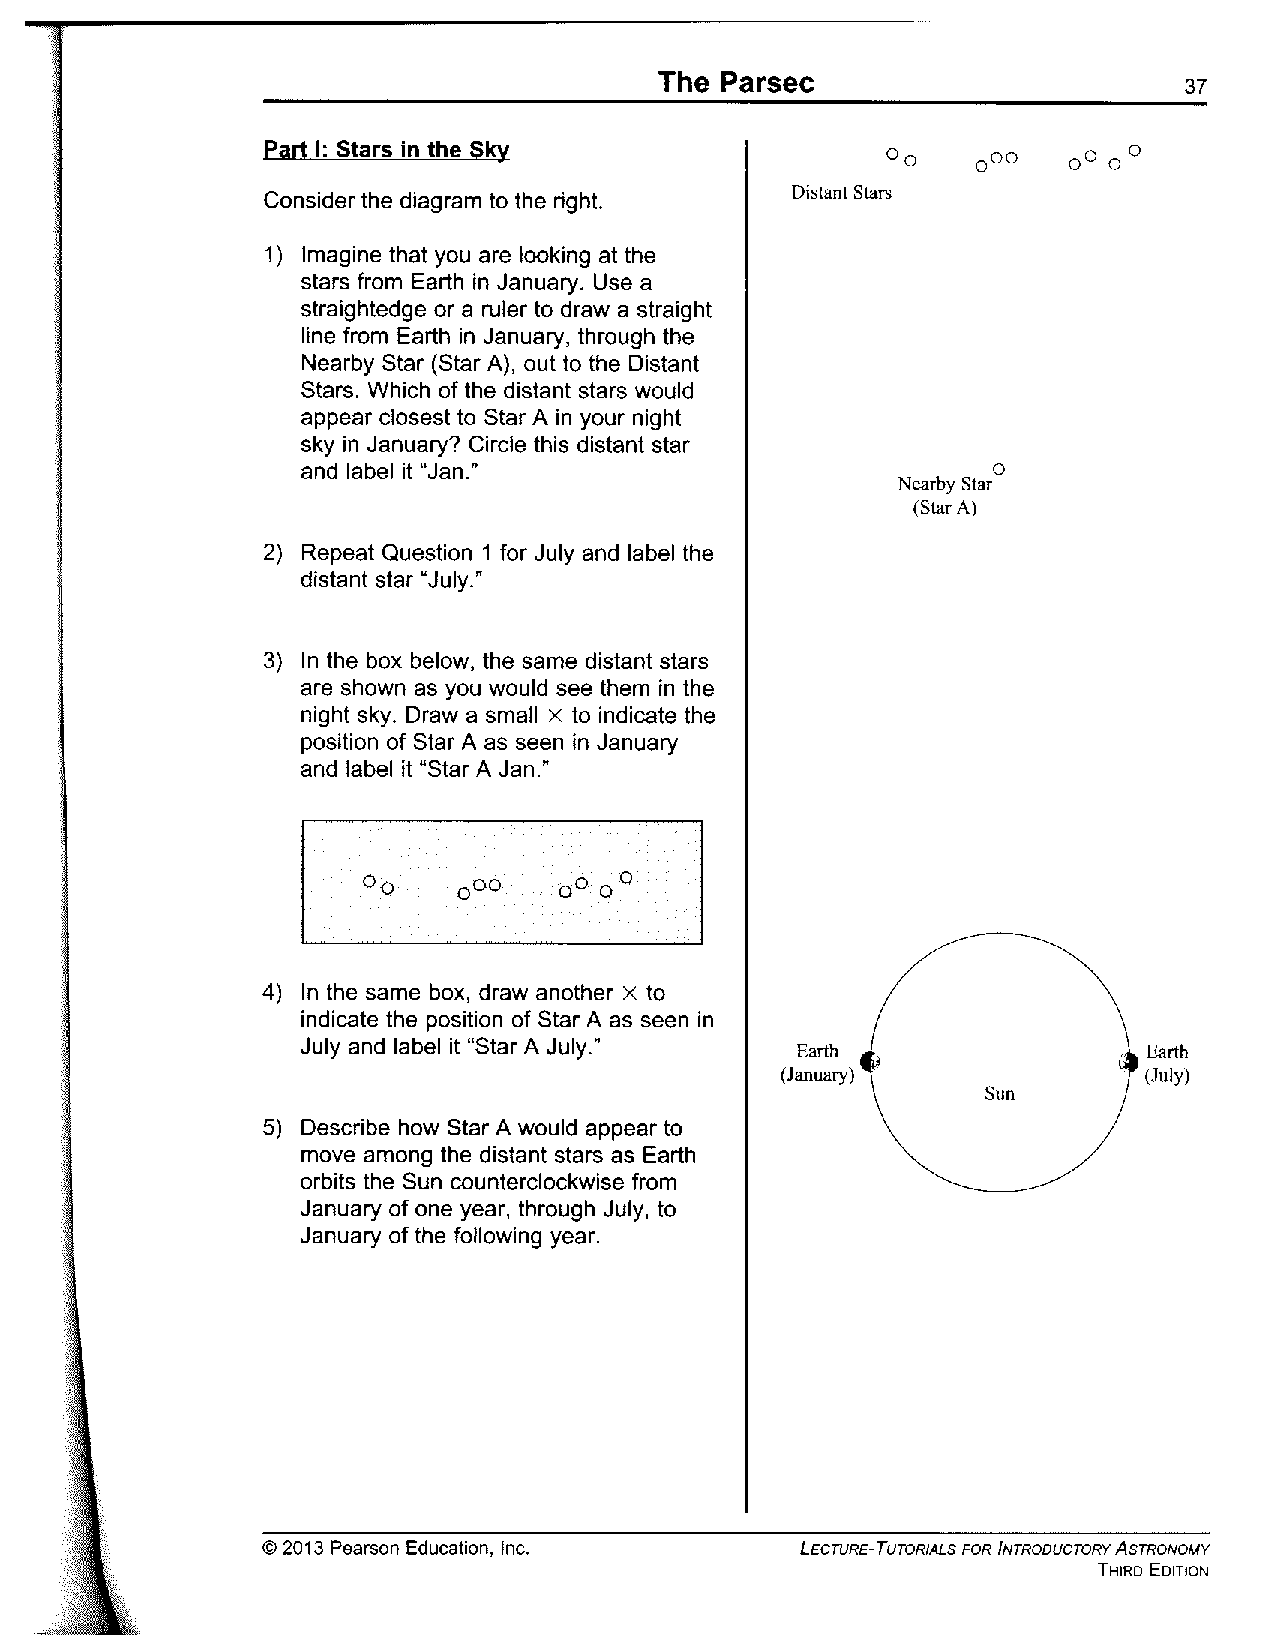
\includepdf[pages=1-2]{parallax/out.pdf}

\section{A quick measurement with hand tools}

You will now use the parallax technique to measure the distance to an object in your environment without needed to travel to it.

\begin{steps}
	\item Identify an object to be your ``nearby star'' and another as your ``distant star'', by analogy to the figure in the worksheet. Also choose the positions to view from as ``Earth (January)'' and ``Earth (July)''. When picking the stars and your Earth positions, check to see that from each Earth position, the distant star does not appear to move much, compared to the nearby star, and your guessed distance to the nearby star is at least 10 times greater than the distance between your two Earth positions.
\end{steps}
	
You'll first use crude measuring tools to compute the nearby star's distance with the parallax technique, and then use a more precise method. First, you'll use the little finger on your outstretched arm as a measurement of angular size --- the width of the index finger covers (``subtends'') about 1 degree.

\begin{steps}
	\item Identify an object to be your ``nearby star'' and another as your ``distant star'', by analogy to the figure in the worksheet. Find a place where you can stand and move a meter or two side to side and still see both ``stars''. The movement will simulate the Earth moving from its January to its July position. When picking the stars and your Earth positions, check to see that from each Earth position, the distant star does not appear to move much, compared to the nearby star, and your guessed distance to the nearby star is at least 10 times greater than the distance between your two Earth positions.
	
	\item Looking from just one eye, move so that the two stars appear to be directly overlapping. Mark your current position as Earth (January). Hold up your smallest finger at arm's length and move to your left or right until your finger fits just in between the two stars. This means that they are 1 degree away from each other in angular separation. Mark this position as Earth (July).
	
	\item Draw a diagram, similar to the second figure in the worksheet, and find your own Earth-Sun distance (half the distance between your Earth positions). Calculate the parallax angle in radians, which is half the 1 degree you measured with your finger. For the distance measurement, you can use a ruler, measuring tape, or objects that have standard lengths like coins, paper money, or sheets of paper (or Google Maps if the distance is very long, like for mountains or tall buildings in the distance).
\end{steps}
	
Now the distance to the nearby star can be found using the triangle formed by the line segments Sun-Earth, Earth-Star, and Star-Sun (see Figure~\ref{par:fig:figure}). Trigonometry relates these lengths to each other according to
\begin{equation}
	\tan p = \frac{a}{d}\,,
\end{equation}
where $p$ is the parallax angle in radians, $d$ is the distance to the star, and $a$ is half of the distance between the two measurement positions. Since the length $d$ is much greater than $a$, the angle $p$ is very small, and so we can use the small angle approximation $\tan u \approx u$, and therefore
\begin{equation}\label{par:eq:pad}
	p = \frac{a}{d}\,.
\end{equation}

\begin{figure}
	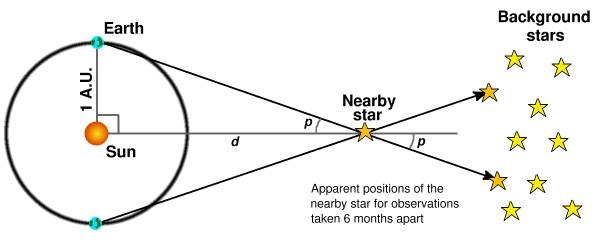
\includegraphics[width=\textwidth]{parallax/parallax-figure}
	\caption{Illustration of the geometry involved in a parallax measurement to determine $d$, the distance to a nearby star.}\label{par:fig:figure}
\end{figure}

\begin{steps}
	\item Use Equation\ \ref{par:eq:pad} to calculate the distance to the nearby star.
	
	\item Conduct the data collection twice more to get two more Earth-Star distances. You can use this to calculate the \textit{measurement uncertainty} --- the uncertainty is half the range of values, and the distance is the average of the 3 distances you found.
	
	\item Find the distance to the nearby star in a more direct way --- measure the distance with a measuring tape or pieces of paper, or for more distant objects, find them on Google Maps.
	For this value, also measure this distance 3 times and find the value and uncertainty as in the previous step.
\end{steps}

\begin{framed}
	\textbf{Notation for uncertain values}
	
To be precise about how imprecise our measurements are, scientists often express the quantities as ``$\langle \textrm{value} \rangle \pm \langle \textrm{uncertainty} \rangle$'', followed by the units. For example, if you measured your average distance to be 3.3 meters, and your uncertainty of that distance to be 0.4 meters, then to express in a succinct way, you can write the distance as ``$3.3 \pm 0.4\:$meters''.
\end{framed}

One way of describing how different two values are, without considering the uncertainty of those values, is to calculate the percent difference:
\begin{equation}
\textrm{percent difference} = \frac{d_1 - d_2}{\left(\frac{d_1+d_2}{2}\right)} \times 100\%
\end{equation}

\begin{steps}	
	\item How close is your parallax distance measurement to the direct measurement? Report the percent difference.
\end{steps}

In the next section, you will compare these values with each other using their uncertainties as well.

%Go out into the third floor hallway of KPTC (the long corridor near room 311).
%Go to the fifth floor of Eckhardt Research Center. Near the elevators on the north side, there are
%two telescopes%
% at the near end of the hallway, and an observing target is located at the far end.
%The target is a mock-up of the night sky, but with colors and relative sizes of objects greatly exaggerated to facilitate observations.

\section{Measuring with more precise equipment}

Using a finger for measuring angular separation is not very precise. Here you'll use the parallax technique to determine the same distance to the nearby star, but using a camera and analysis software instead.

%You will now use the telescope apparatus to measure the parallax of a “foreground star”
%(actually a ball on a stick)
%(actually a nearby building), with the
%mock-up star field
%Chicago skyline
%serving as “background stars.”
%Place the “foreground star” part way down the hallway between the telescopes and the observing target.
\begin{steps}
	\item Take a picture from a digital camera (likely your phone camera) from the vantage point of each Earth position used above.
	
	
%Make sure that it is positioned so that sightlines from both telescopes
%pass through both the “foreground star” and the “background stars,”
%(an overlapping background of the skyline).
%With your smartphone, take an image of the “foreground” and “background” stars through each telescope.
%Also measure the distance between the two telescopes using a measuring tape and record
%this value in your lab notebook. See Figure~\ref{par:fig:images} for example data.

%\begin{figure}
%	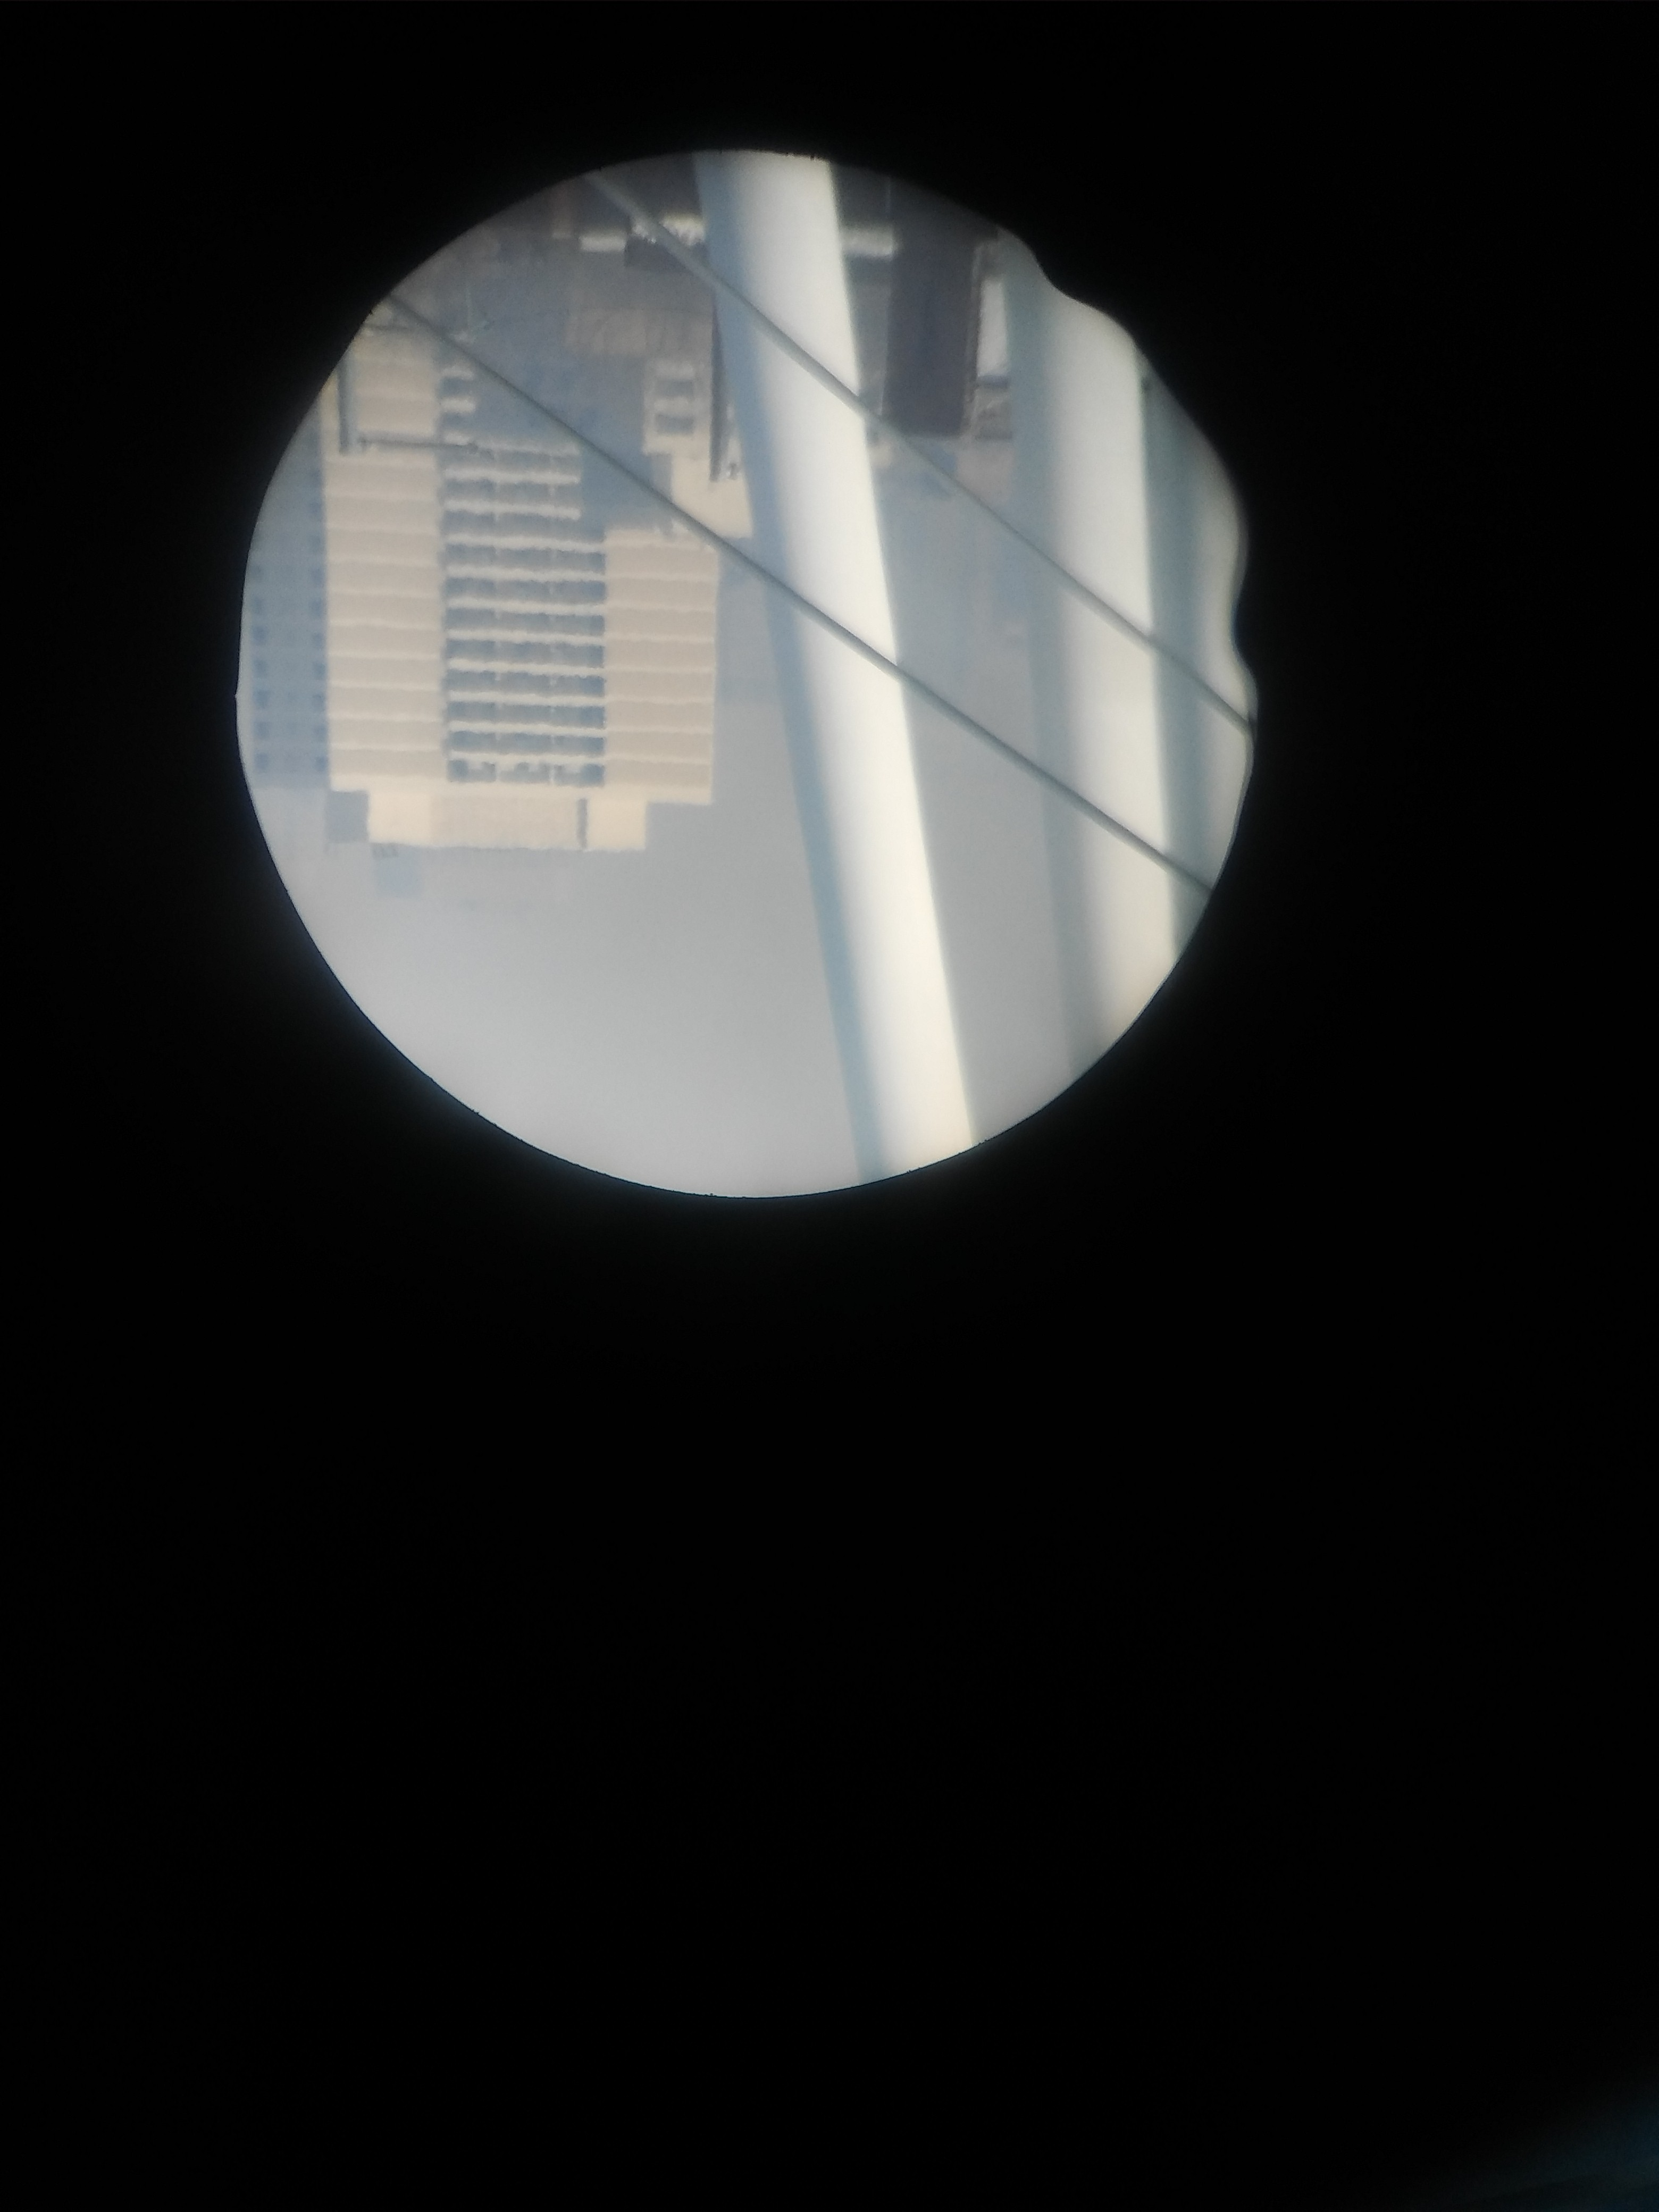
\includegraphics[width=0.5\textwidth]{parallax/parallax-image-1}
%	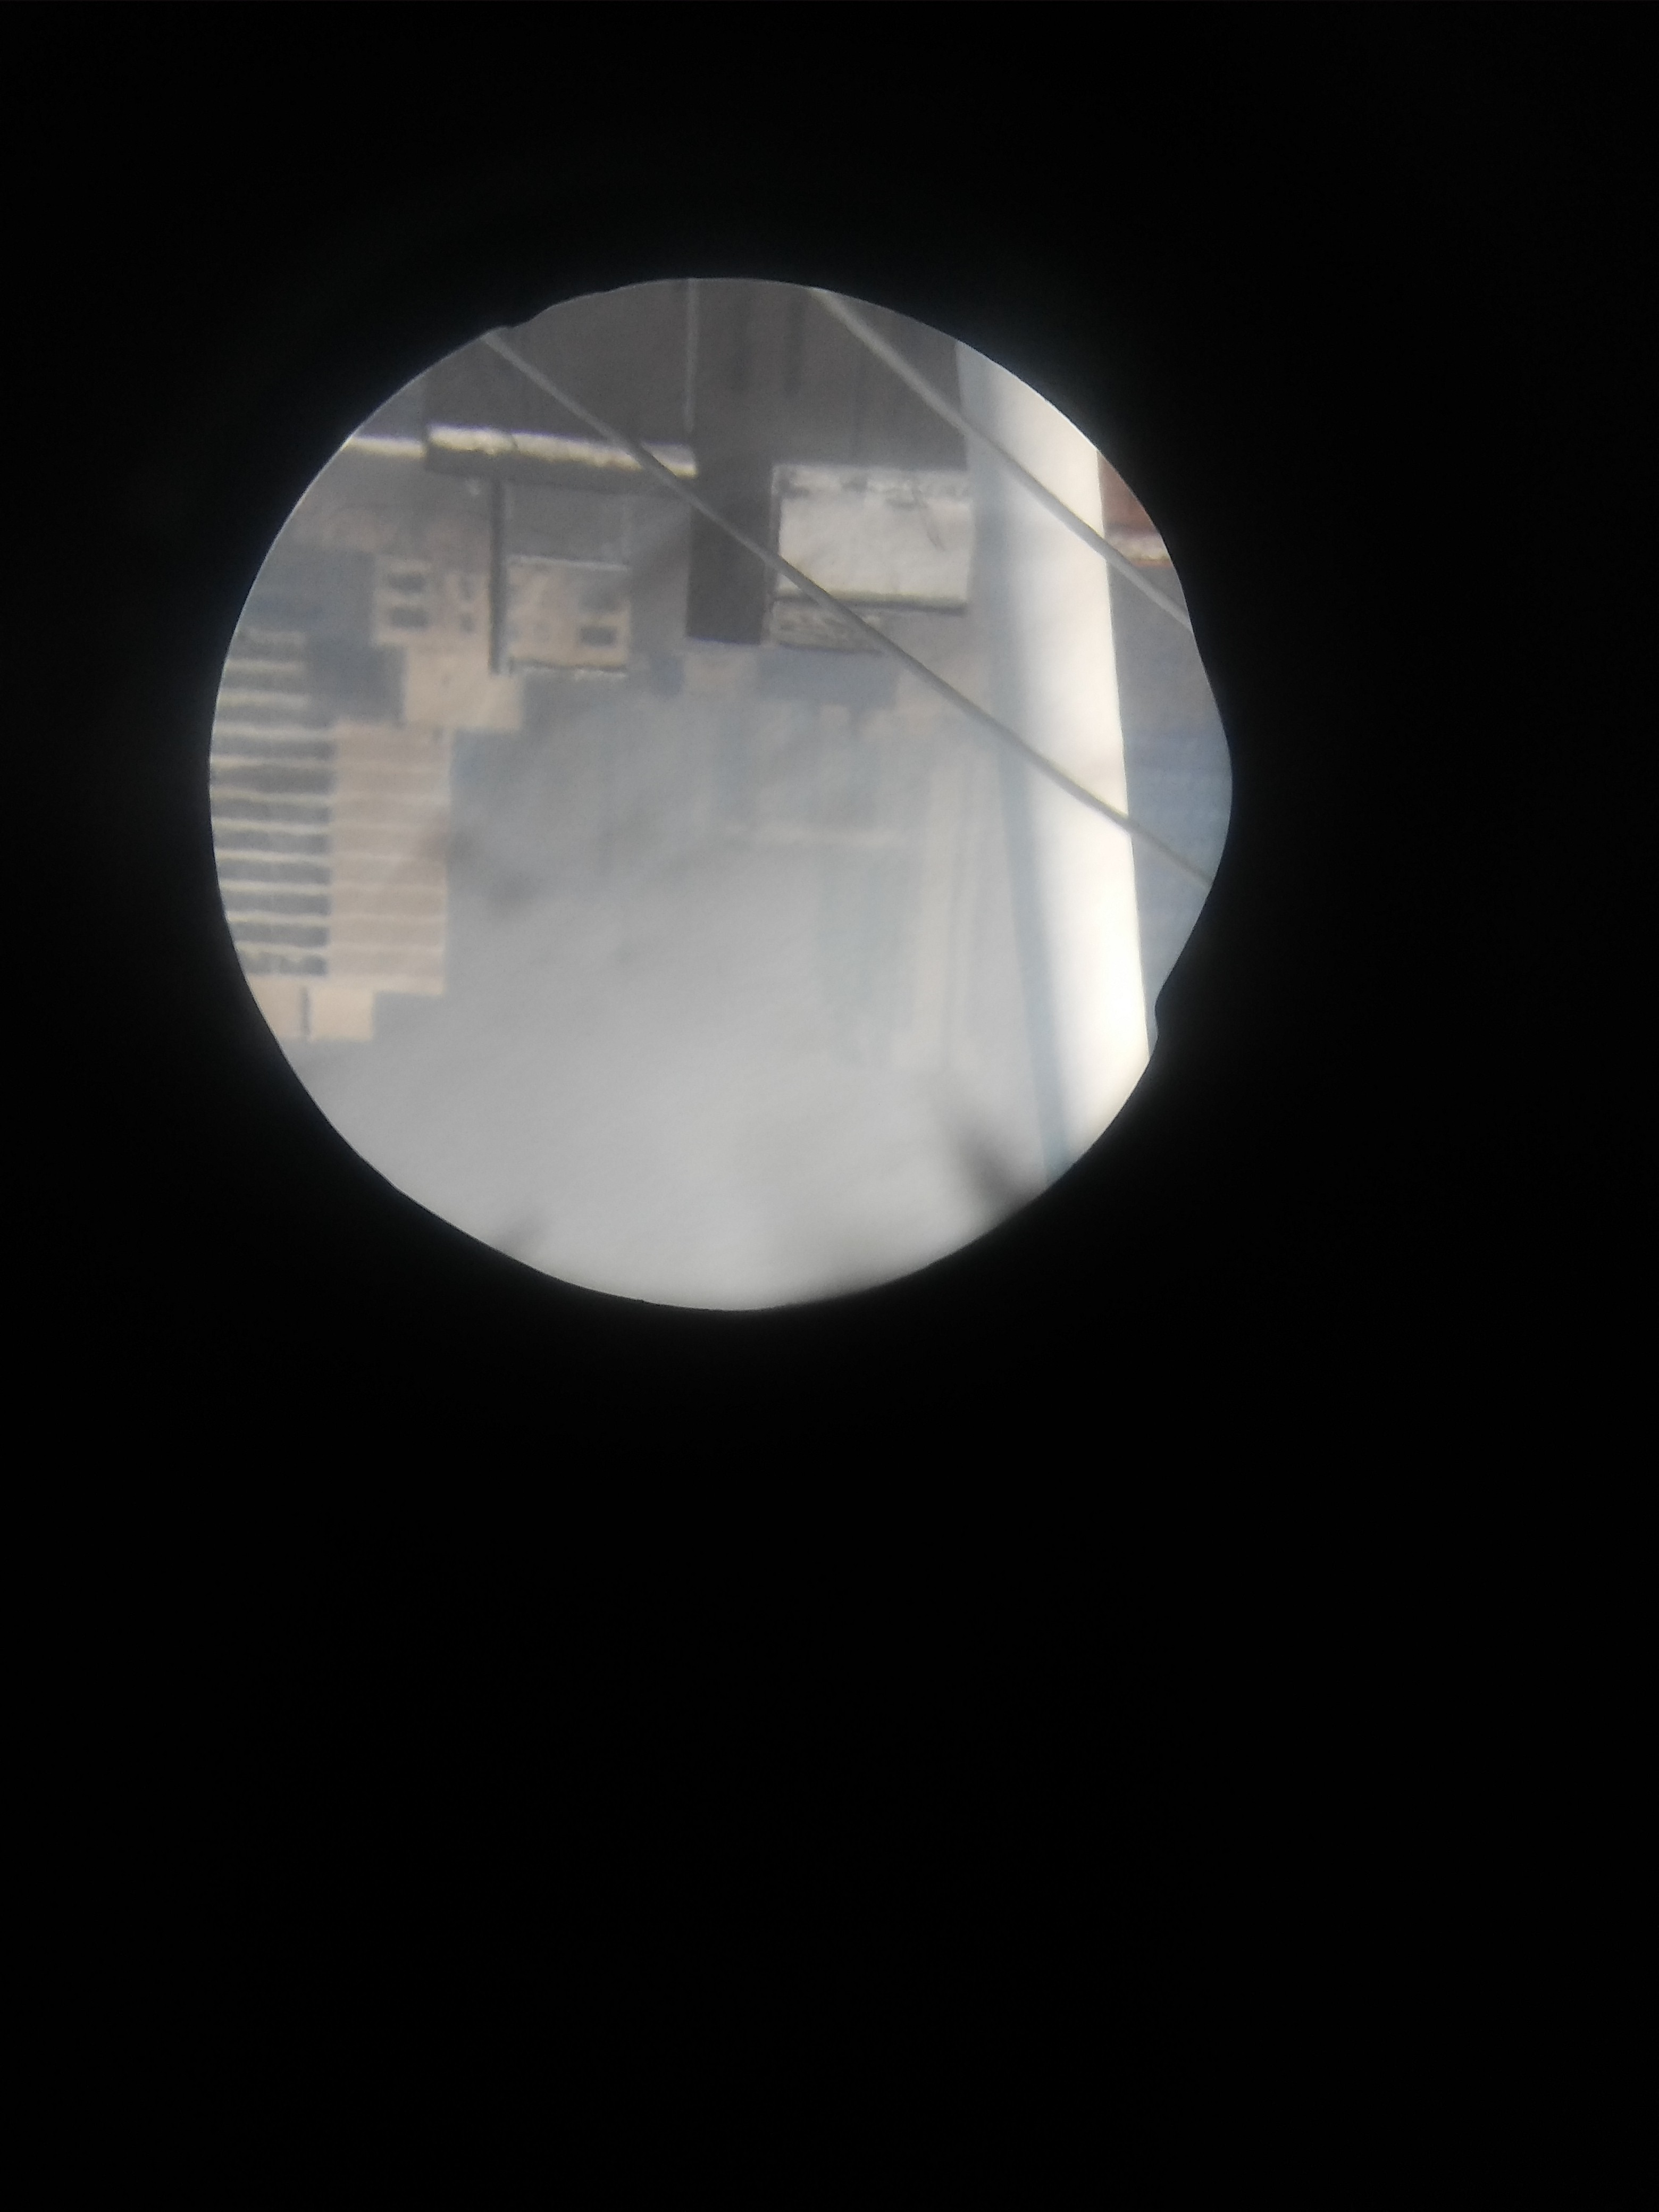
\includegraphics[width=0.5\textwidth]{parallax/parallax-image-2}
%	\caption{Example images. My foreground ``star'' was the point defined by the left intersection of the lower cable and the white pillar on top of the gym on campus. One of my reference ``stars'' was the top right corner of the building in the background. Note that the images produced by this telescope are upside down.}\label{par:fig:images}
%\end{figure}

%You have now finished collecting data, so now it’s time to analyze it. 
	\item Upload your photographs to a computer. The simplest way to do this may be to email the images to yourself from your phone. Give each file a descriptive name (e.g. ``\texttt{parallax\_left\_telescope}'').
\end{steps}

\subsection{Finding the pixel scale}

Notice that with the finger, I told you that your little finger, outstretched, is about 1 degree wide. This was a conversion between the linear size of your finger, for example 1 cm, to an angular size, 1 degree. With the camera, we need to find out the similar conversion --- how many pixels in an image corresponds to what angular size, also known as the \textit{pixel scale} of the image. To do this, you can take a known angular size and measure its length in pixels.
\begin{steps}
	\item Find an object of known length and place it a known distance from the camera (distance to camera should be 10 times or more the length of the object). Take a picture of that object.
\end{steps}

You will now convert the images from their default format (likely .png or .jpeg) into .fits
files, a format commonly used by astronomers. This format will be readable by SAO
Image DS9, an astronomical image analysis tool.
\begin{steps}
	\item Convert the image files to a .fits format using your favorite image processing software, or the software ``GIMP'' (Gnu Image Manipulation Program), or an image conversion website like \url{https://www.files-conversion.com/image/fits}. For using GIMP, open the file. From the FILE menu, select EXPORT AS, change the
file extension to “.fits,” and then click EXPORT. Repeat this procedure for each of your
images.

\item Open a saved .fits image of the pixel scale image in DS9. Your first task is to measure the pixel scale.
%Adjust the contrast so you can clearly see the field of view.
From the menu at the top of the screen, select REGION, SHAPE, LINE. On the first row
of buttons in the DS9 window, click EDIT then on the second row click REGION. Draw
a line along the known length of the object. On the first row of buttons, click REGION then on the
second row click INFORMATION. A window should pop up that will give you the length
of the line in physical units, that is, in pixels. \textbf{Record this value in your lab notebook.}

\item Find the angular size of the known object. Since the object is far away, we can again use the small angle approximation for the triangle involved and find that the angular size of the object is equal to its length divided by the distance to the object. This angle is in radians.

\item Find the pixel scale by dividing the number of pixels in the length by the angular size of the known object. This gives the pixel scale in pixels per radian.

\end{steps}
\subsection{Finding the parallax angle}

Now that you have the pixel scale of the image, you can use that to measure the parallax angle of the your nearby star and thus find the distance to that object like you did with the little finger method.

\begin{steps}
	\item Open the first parallax image. Measure the displacement from the nearby star to the distant star. Convert that displacement to radians using the pixel scale. Make sure to record both the X- and Y- offsets. Repeat these measurements for the second parallax image using the same distant star.

	\item Find the total angular distance the star moved between images. To do this, subtract the X- offsets from each other, and subtract the Y- offsets from each other. Then use the Pythagorean theorem to find the total distance moved ($d = \sqrt{x^2 + y^2}$). Divide this by two to get the parallax angle.
	
	\item Use Equation\ \ref{par:eq:pad} to find your new calculation for the distance to the nearby star.
	
	\item Calculate the percent difference between this and the direct measurement like you did in the previous section.
	
	\item Use the $t'$ statistic described in Appendix\ \ref{unc:sec:comparing} to compare the two values and interpret the result --- do these two ways of distance measurement really measure the same thing?
\end{steps}

%Given that the field of view of the Galileoscope is 1.5\textdegree
% (0.75\textdegree with the Barlow eyepiece)
%calculate the \textit{plate scale} of your images, in arcsec/pixel.

%Select a reference star from your parallax measurements. Using your plate scale,
%determine the angular separation between the reference star and the target star. Record
%the value for the total separation, $r$, and for both the horizontal ($x$) and vertical ($y$) components. You can
%check your measurements against each other by inputting these values into the
%Pythagorean formula: $r^2 = x^2 + y^2$. Do your measurements agree?
%
%Repeat the above calculations for all reference stars in both of your parallax images. You
%can now calculate the distance to the foreground star. The distance to a star can be found using the triangle formed by the line segments Sun-Earth, Earth-Star, and Star-Sun (see Figure~\ref{par:fig:figure}). Trigonometry relates these lengths to each other according to
%\begin{equation}
% \tan p = \frac{a}{d},
%\end{equation}
%where $p$ is the parallax angle in radians, $d$ is the distance to the star, and $a$ is half of the distance between the two measurement positions. Since the length $d$ is much greater than $a$, the angle $p$ is very small, and so we can use the small angle approximation $\tan u \approx u$, and therefore
%\begin{equation}
%p = \frac{a}{d},
%\end{equation}



%Use each reference star to calculate an independent measurement of parallax. To do this, for each reference star, you'll need to find how far (in radians) the target star has moved between the two observations. Using vector arithmetic\footnote{See \url{https://www.mathsisfun.com/algebra/vectors.html} for a short tutorial}, subtract the two displacement vectors from each other by components and find the magnitude of that difference vector. Divide by 2 and convert to radians to find $p$. After finding $p$ from each reference star, average these values together and estimate your uncertainty by finding the standard deviation of these measurements. You can perform this calculations in Excel using the functions AVERAGE() and STDEV(). Report your measurements in a table in your lab
%report.
%
%Also use a map to find the distance from you to your foreground star (with uncertainty). Compare these quantities with their uncertainties using the procedure found in Appendix~\ref{unc:sec:comparing}, to see the degree to which they agree.

%\section{Questions}\label{par:sec:questions}
%
%These should be included in your lab report.
%
%\begin{steps}
%	\item Your parallax measurements depend on an incorrect implicit assumption. What is
%	this assumption, and how will it bias your results? How would you change the
%	procedure in order to minimize this bias?
%	\item What were the primary sources
%	of uncertainty? How would you improve the procedure for future measurements?
%\end{steps}

\section{Report checklist}

Include the following in your lab report. See Appendix~\ref{cha:lab-report-format} for formatting details. Each item below is worth 10 points.

\begin{enumerate}
	\item Your group's agreements about communication.
	\item The completed worksheet ``The Parsec''.
	\item Work and final answer for your distance measurements using your finger, with uncertainty.
	\item Work and final answer for direct distance measurement, along with percent difference.
	\item A figure with your three images (pixel scale image and two parallax images).
	\item The displacement vectors from distant star to nearby star.
	\item Final determined value of the distance and comparison with the direct distance using percent difference and $t'$ statistic. Show your work (see Appendix~\ref{cha:lab-report-format}).
%	\item Answers to the questions in Section~\ref{par:sec:questions}, with justification.
	\item A 100--200 word reflection on group dynamics and feedback on the lab manual. Address the following topics: who did what in the lab, how did you work together, how group roles functioned, what successes and challenges in group functioning did you have, and what would you keep and change about the lab write-up?
\end{enumerate}
\chapter{Peculiarities of light: doppler shift, spectral lines, and limits of resolution}


\chapter{Rotating solar systems and radio astronomy}

\section{introduction} 
You would think that being limited to radio signals, the kinds of observations you could make and the information you could gather would be relatively small. In fact, there are a wide range of observations and interesting phenomena which can be detected using a radio telescope. From the elemental make up of a distant planet's atmosphere, to the detection of extreme astronomical objects. In fact, we can use observations of signals from hydrogen clouds in the galactic plane and, using the knowledge we gained of the Doppler shift, obtain an estimate for the distribution of matter in the Milky Way. By now you know how to go from radio signals to velocity, but how do you go from velocity to mass? In this lab, not only will you learn how we can estimate mass distribution, but you will also learn the basics of using the Small Radio Telescope. 

\section{Learning Goals}
\begin{itemize}
	\item Make predictions about large, gravitationally bound systems based on observations of smaller scale systems.
	
	\item Make observations using the Small Radio Telescope (SRT) and interpret the data
	
	\item Calibrate the SRT and understand the uncertainty by measuring background noise in the Chicago sky 
\end{itemize}

\section{Masses and Orbital Velocity} %working title only
One of the main labs you will carry out this quarter is a measurement of the motion of the Milky Way using the SRT. It is important that when you make these measurements that you understand the results you obtain. In this experiment, you will learn how the specific observations you will make can be used to make some predictions about the milky way. 

\subsection{Goal}
Learn how new phenomena can be predicted or inferred from basic physical principles and how to interpret rotation curves. 

\subsection{Equipment}

\begin{itemize}
	\item Desmos Graphing Calculator: https://www.desmos.com/calculator
\end{itemize}

\subsection{steps}

\begin{steps}
	\item First, we know from Newton's first law that the force on an object is equal to its mass times its acceleration, $F=ma$. We also know that an object moving in a circle will experience an acceleration towards the center of its path which is given by $a = \dfrac{v^2}{r}$, where $v$ is the velocity of the object and r is the radius of its path. Using these two equations, find an equation for the force experienced by an object undergoing circular motion. 
	
	\item Objects in orbit also move in an approximately circular path and the force of gravity they experience is given by $F = G\dfrac{Mm}{r^2}$, where M and $m$ are the masses of the two objects and $G$ is the gravitational constant. Using the equation you found in the previous step, derive an equation for the velocity of the orbiting object as a function of its radius.\textit{Remember to cancel out like factors. Your equation should be in terms of M, r, and G}
\end{steps}

Below you will find what is known as a \textit{rotation curve}, which plots the orbital velocities of objects in an orbital system against their distance from the center. Using these curves, it is possible to learn a lot about the system it describes. 

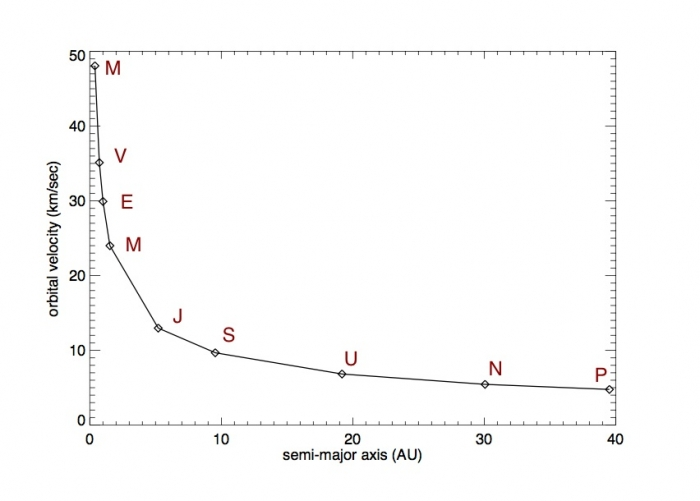
\includegraphics[scale = .7]{srt-background-rotation/keplerian-orbit.jpg}

\begin{steps}
	\item Describe the graph  that you see. How does velocity change as you move away from the center of rotation? \textbf{Write your answer in the lab report}
	
	\item This rotation curve can be modeled by the equation you found above. How would you manipulate the equation to obtain the curve. What variables would have to change? Which values would remain the same? \textit{It might help  to use the graphing calculator provided in the link above} \textbf{Write your answers down}
	
\end{steps} 

When you first derived the equation for rotational velocity, you assumed that $M$ represented the mass for a single object. Now assume that it represents the total mass contained within the orbital radius. 

\begin{steps}
	\item Given the above rotation curve, how does the mass contained change as you move farther from the center of the orbital system? Does it change? What does this tell you about the distribution of mass in the orbital system?
\end{steps}

Now we will take a look at curve B from the graph below
	
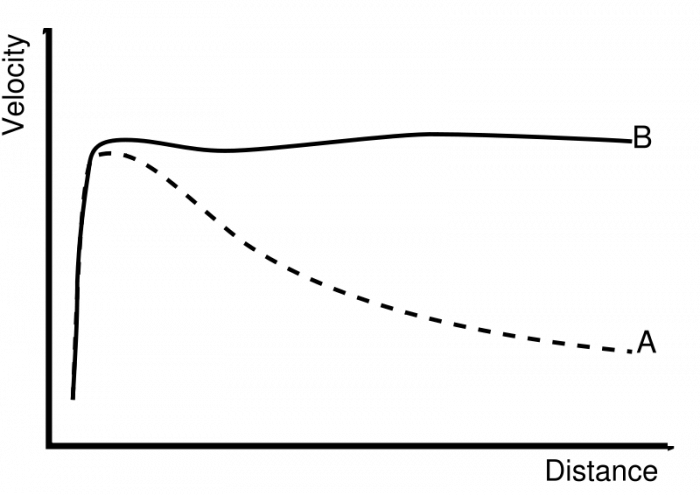
\includegraphics[scale = .5]{srt-background-rotation/galactic_rotation_curve}

\begin{steps}
	\item Following a similar process to what you used for the first curve, what changes would you have to make to obtain curve B so that velocity remains constant. \textit{Specifically, how would M have to change with respect r to make v constant}
	
	\item Based on your answer to the previous question, what does curve B tell you about the distribution of mass in the orbital system? 
	
	\item Now, look up information on the masses of the planets in the solar system as well as the sun. Which of the two rotation curves would you expect the solar system to have? \textit{It might help to add up all the masses and see how much each planet contributes to the total mass}
	
\end{steps}
	


\section{Background Noise} %working title only
While learning about the theory behind making astronomical observations is always useful, the best way to gain an intuition for these concepts is through hands on experience. For this experiment, you will learn how to operate the small radio telescope located on top of the Eckart Research Center. In particular, you will learn how to calibrate the telescope and measure the background noise present in the Chicago sky.

\subsection{Data Output} 

When using the telescope you will notice that it outputs a temperature. This is not that the SRT is actually measuring the object's temperature, rather, it is simply interpreting the power it receives as a temperature. Similarly, when calibrating, the telescope will display a system temperature $T_sys$ which interferes with our measurements. When calibrating, we account for $T_sys$ and it is subtracted from our measurements. 

\subsection{Telescope Control}
Unfortunately, you will not be able to directly control the telescope and it will instead be controlled by a designated telescope technician. However, you should still learn the basics of controlling the telescope so you can give the technician proper observation instructions. In this case, the technician will act as your hands when operating the telescope, inputting the commands you give them.

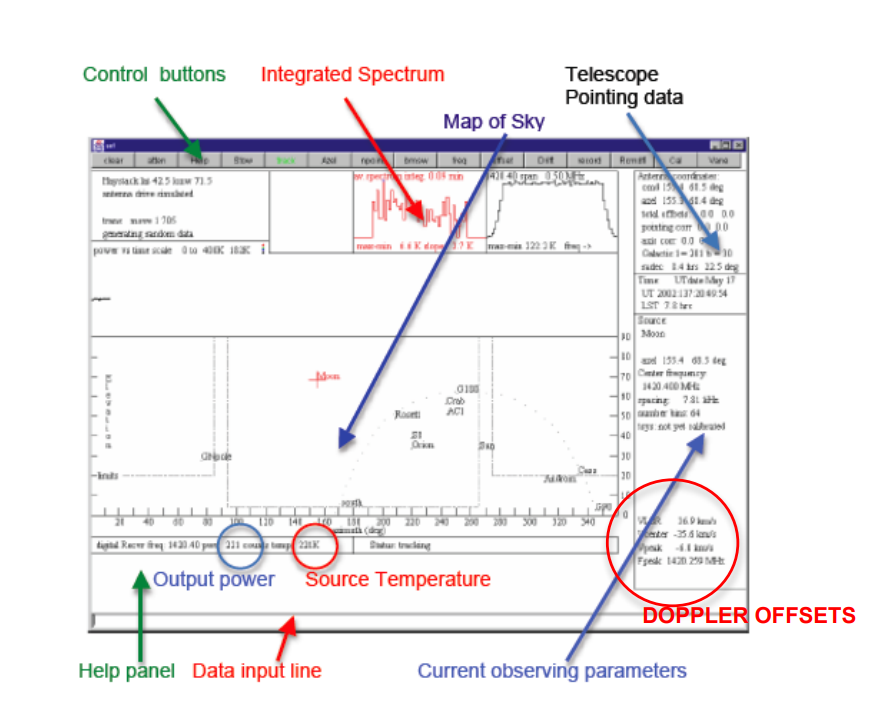
\includegraphics[scale = .9]{srt-background-rotation/display_diagram}

\subsection{Control Buttons}
The control panel display has a line of control buttons at the top that set
up a command for the telescope. For instance, if you want to change the receiver
frequency, you click on the “freq” button. Instructions and help information are
then displayed in the help panel below the map while the cursor is pointed to the
button (This field is blank when you move the cursor away). If you want to
change the frequency, then type data into the data line (e.g. “1420.4 4”), click
“enter” or “return”. Be sure you leave a space between 1420.4 (which is the
frequency) and the number 4 (which sets the bandwidth of the system). The
current observing parameters will be updated in the appropriate box.

\subsection{Control Display \& Sky Map}
The control panel shows a map of the current sky in Azimuth and
Elevation units. 0 degrees azimuth points North, 90 degrees points East, 180
degrees points South and 270 degrees points West. The horizon is at 0 degrees
elevation and Zenith is at 90 degrees. The telescope can point to about 85
degrees in elevation.
The map displays objects visible at the current time. The software tracks
an object or a given azimuth and altitude position, including corrections for the
rotation of the earth. Also displayed on the map are various individual
astronomical sources and a track of dots that show the plane of the Milky Way.
The Longitude of points along the equator of the Milky Way are shown as Gxxx,
where xxx is the Galactic longitude. We have an unobstructed view of all objects
above about 20 degrees.

\subsection{Pointing the Telescope}
You can point to any given position in the sky by clicking on the “AzEl”
button and then typing the desired Azimuth and Elevation in the command line at
the bottom of the display. (e.g., 30 45 “enter” will send the telescope to a position
of 30 degrees azimuth and 45 degrees elevation). When you enter a position you
will see a yellow cross and the CMD numbers will change to these numbers. 

When “track” shows up in green at the top of the display, the telescope has
acquired the position and is tracking it, this holds for sources. If the telescope
does not move, then you probably have to click on “track”.
Occasionally the telescope motor will get stuck and stall. Normally it fixes
itself automatically by going back to the “Stow” position (where it is stowed after
every observation), but if it remains stalled for several minutes click “Stow” to do
so manually. This can be a nuisance and time-consuming but you should still be
able to obtain the necessary data if this happens.

\subsection{Steps}
\begin{steps}
	\item Set the receiver frequency to 1416MHz. At this frequency, you will detect the continuum radiation. That is, radiation emitted relatively uniformly over a broad band of frequencies  
	
	\item Point the telescope at a position in the sky away from the galactic plane. Do this by choosing Azimuth and Elevation (AzEl) coordinates which do not lie in the arc of labeled locations on the telescope display. \textbf{Record these coordinates}
	
	\item Once the telescope has reached the given position, click ``Clear'' to erase any previous reading. Record the raw temperature displayed. Then click ``Cal'' to calibrate the telescope. \textbf{Record the new output temperature.} 
	
	\item Repeat the calibration a few times until you read a stable system temperature $T_{sys}$. Wait around 1 minute between calibrations
	
	\item After you have successfully calibrated the telescope, from you calibration position, point the telescope 15 degrees lower in elevation and calibrate the telescope 2-3 more times. \textbf{Record $T_{sky}$ and $T_{sys}$ as well as the telescope coordinates}
	
	\item Returning to your original pointing elevation, repeat the above step but this time changing the azimuth by 50 or 75 degrees.
	
	\item From your observations, how uniform is the sky in Hyde Park? \textbf{Include a table of your measurements and a discussion of the question in your report.}
\end{steps}
\chapter{How fast is the galaxy rotating and what does it mean?}

\section{Introduction}
Throughout the past few weeks, you have been preforming labs which at times might have seemed disparate or only somewhat connected to each other. Now, you will bring all these concepts you have been working with in order to perform observations and make conclusions regarding the motion of the Milky Way. In this lab, you will be trying to measure how the rotational velocity of the milky way varies changes as you move away from the center. However, given the scale of the Milky Way, there is no way for us to directly observe its motion. However, we can use the motion of objects within the galaxy to calculate its rotational velocity. One useful object to do this are hydrogen clouds. In a previous lab you learned how shifts in frequency can be used to calculate the velocity of an object. In the case of hydrogen clouds, given that they emit at a very definite, known frequency we can calculate their velocity to a very high degree of accuracy. Moreover, given how common they are throughout the Milky Way, they can be used to make these measurements at many different points along the galactic plane. Using this data, you will calculate the rotational velocity of the galaxy at that point and create a rotation curve for the Milky Way. You will then use the curve to make inferences about the mass distribution of the Milky Way and see why dark matter is believed to play a role in its structure. 

\section{Learning Goals}
\begin{itemize}
	\item Use observation of hydrogen cloud velocities to determine motion of galactic plane
	
	\item Organize and present data in a logical and consistent manner and draw conclusions from it
	
	\item Interpret rotation curve data in order to make inferences about the mass distribution in the Milky Way
\end{itemize}

\section{Team roles}

\textbf{Decide on roles} for each group member. The available roles are:

\begin{itemize}
	\item Facilitator: ensures time and group focus are efficiently used
	\item Scribe: ensures work is recorded
	\item Technician: oversees apparatus assembly, usage
	\item Skeptic: ensures group is questioning itself
\end{itemize}

These roles can rotate each lab, and you will report at the end of the lab report on how it went for each role. If you have fewer than 4 people in your group, then some members will be holding more than one role. For example, you could have the skeptic double with another role. Consider taking on a role you are less comfortable with, to gain experience and more comfort in that role.

Additionally, if you are finding the lab roles more restrictive than helpful, you can decide to co-hold some or all roles, or think of them more like functions that every team needs to carry out, and then reflecting on how the team executed each function.

\section{Rotation of the Milky Way}

\begin{figure}
	\centering
	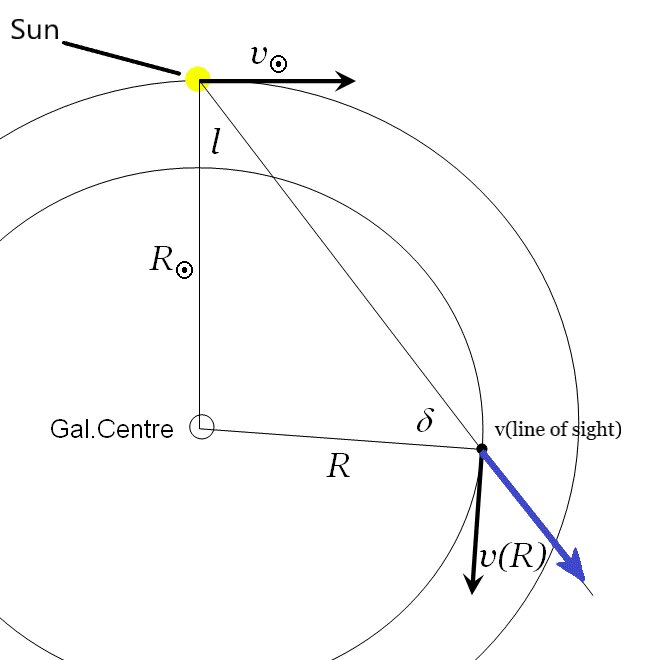
\includegraphics[width = 0.7\textwidth]{srt-galaxy-rotation/geometry_edit}
	\caption this
	\label{sgr:fig:gal-geom}
\end{figure}

\subsection{Calculating Rotational Velocity}
When measuring the velocity of these objects, we have to keep in mind that we are moving relative to them. As such, we are not measuring their rotational velocity directly, but their velocity relative to us. We therefore have to do several calculations to get their orbital velocity. To do this calculation, we will need several components. First, we will need the velocity of the sun in the line of sight for the galactic longitude $l$. This is because the Sun is also moving along the galactic plane, and thus we need to be able to account for it in our measurements. We already know that the radial velocity of the sun is 220km/s, so using some simple trigonometry, we can see that the line of sight velocity is given by $$V_\textrm{sun}(l) = 220\:\mathrm{km}/\mathrm{s}\sin(l)$$ We also need to account for Earths rotation around the sun as well as relative motion of the solar system. This is given to you by the SRT as the VLSR or Velocity relative to the Local Standard of Rest. From the graph generated by the telescope, we simply need the maximum VLSR, as it corresponds to the hydrogen cloud directly in our line of sight. The circular velocity of the cloud can thus be obtained by  $$V_c(r) = v_\textrm{max} (l) + v_\textrm{sun}(l)$$ Finally, for the final data processing, you will need the distance of that cloud from the center of the galaxy. Once again, from the geometry of the graph above, we can see that this can be found from the distance of the Sun to the center $r_0 = 8.5\textrm{kpc}$ (kiloparsec) and the galactic longitude $l$. The distance is then given by $$r = r_0 \sin(l)$$


% Change gamma to l, parenthesis around 220km, spacing between number and unit use example on slack



\subsection{Goal}
Measure the rotational velocity of the galactic plane along different orbital radii, create a rotation curve for the milky way and infer the mass distribution from it.
\subsection{Equipment}
\begin{itemize}
	\item LAB sky survey: \url{https://www.astro.uni-bonn.de/hisurvey/AllSky_profiles/}
\end{itemize}


\subsection{Calibration}
Before you begin your observations of the hydrogen clouds, you have to calibrate the telescope similarly to how you did in the previous lab. However, this time you have two options for calibrating: The offset frequency method and the off-source method.The two methods are described below

\subsubsection{Offset Frequency Method(recommended)}
\begin{steps}
	\item Move the telescope to one of the locations you want to measure on the galactic plane (marked by the Gxxx)
	
	\item Change the telescope frequency to 1423MHz in mode 4 and clear the screen. This frequency is far enough from the hydrogen line that you will only be measuring the receiver noise and thermal background.
	
	\item Once you have cleared the output, select "Cal" to begin the calibration procedure. Note the $T_\textrm{sys}$ and $T_\textrm{rec}$
	
	\item Clear the output again and repeat the calibration procedure 2-3 times or until you note a stable $T_\textrm{sys}$ and $T_\textrm{rec}$. 
\end{steps}

\subsubsection{Off-Source Method}

\begin{steps}
	\item Point the telescope to some location far away from the galactic plane (away from the labeled sources). 
	
	\item Change the receiver frequency to 1420.4MHz in mode 4 and clear the output
	
	\item Once you have cleared the output, select "Cal" to begin the calibration procedure. Note the $T_\textrm{sys}$ and $T_\textrm{rec}$
	
	\item  Clear the output again and repeat the calibration procedure 2-3 times or until you not a stable $T_\textrm{sys}$ and $T_\textrm{rec}$. \textbf{If there is a major hydrogen source in your pointing, the calibration will not work. Look out for strong spectral features when calibrating to make sure you are not pointed at a hydrogen source. If this were the case, try moving the telescope. You likely wont find a spot without any hydrogen emissions, but you can try to avoid significant sources. If not try the offset frequency method instead.} 
\end{steps}


\subsection{Steps}

\begin{steps}
	\item In the control panel, the positions of different Galactic longitudes along
	the equator are indicated by Gxxx (where xxx is in degrees). If you see
	longitude of 90 degrees and smaller, start at the longitude of 90
	degrees and work your way down to the smallest longitude you can
	observe down to zero of the center of our Galaxy (coincident with the
	source named Sgr A). If you cannot observe longitudes smaller than
	90 degrees observe one or two longitudes that are up in the sky. Note
	that galactic coordinates labeled in the SRT display can be pointed to
	by clicking on them – for the rest you have to estimate (or look up) the
	Az El of the desired longitude on the galactic plane. %add framing comment 
	
	\item Move to your first pointing and press Clear button to clear the spectrum accumulated by the SRT.
	
	\item  Set the frequency to 1420.4MHz with mode  4 by typing in ``1420.4 4'' and obtain the spectrum for the galactic longitudes visible in the sky by integrating for 10--20 seconds (or longer) along the same pointing 
	
	\item After integration click on the spectrum window to get a detailed plot of
	the spectrum in a separate window. You will see emission flux in units of Kelvin (K) as a
	function of frequency and VSLR. Based on your understanding of how frequencies are affected by Doppler shift, estimate that maximum velocity of the clouds visible in the spectrum. 
	
	\item Record the spectrum by taking a screenshot of the spectrum plot. If necessary, crop the image in your preferred image editor such that only the spectrum viewer is visible. Your screenshot should look something like Figure \ref{sgr:fig:spec-example}
\end{steps}

\begin{figure}
	\centering
	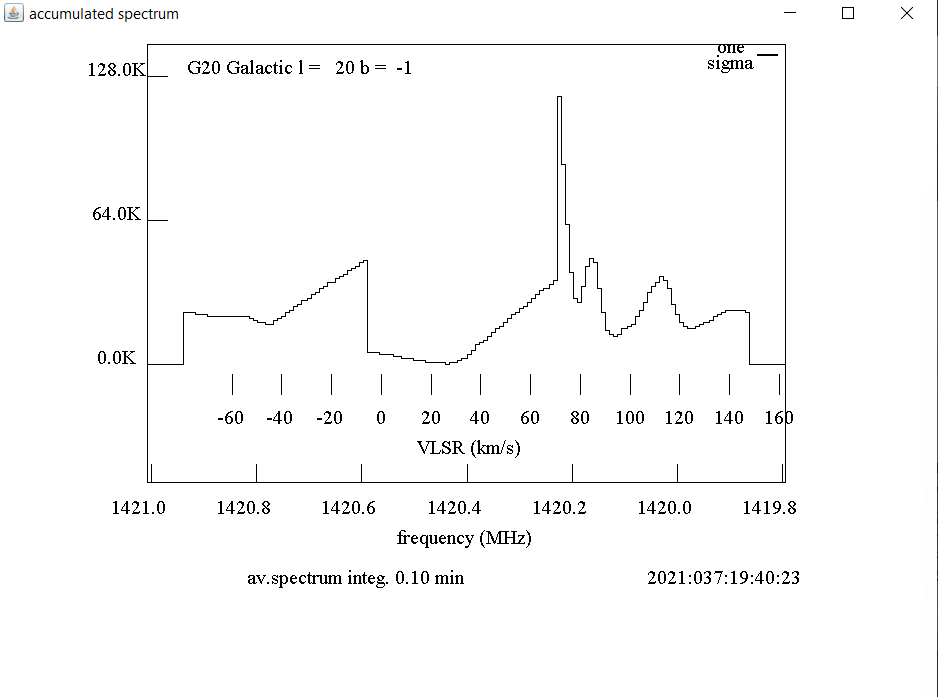
\includegraphics[width = 0.7\textwidth]{srt-galaxy-rotation/spectrum_ex}
	\caption{An example of a good capture of the spectrum plot. Note the clarity of the units, the lack of external elements distracting from the graph, and the inclusion of all relevant information} 
	\label{sgr:fig:spec-example}
\end{figure}

\begin{steps}
	\item Proceed to the next Galactic longitude available for observation. Press Clear button to clear the spectrum before you make observation at
	each new longitude. Record longitude and spectrum. Given the limited time, each group should do 2-3 observations and supplement the rest of the data either by sharing with the other groups or using the LAB survey described below.%rewrite given current situaton
	
	\item After you have preformed all the possible observations, open the link to the LAB sky survey provided in the equipment section. 
	
	\item In the search box, make sure that only the LAB survey box is checked and that Dec is always at 0. Figure \ref{sgr:fig:lab-box} demonstrates how the display should look like
\end{steps}

\begin{figure}
	\centering
	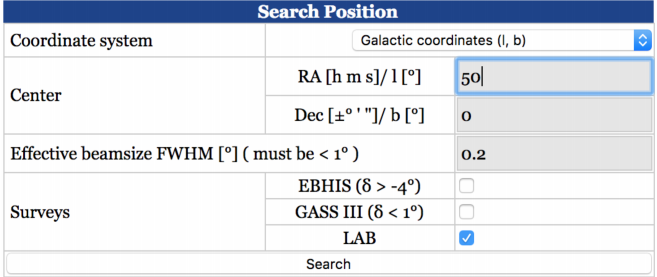
\includegraphics[width = 0.7\textwidth]{srt-galaxy-rotation/LAB_box}
	\caption{The input form for accessing the LAB spectra. Dec is always set to 0, only LAB is selected, FWHM is set to 0.2 and galactic coordinate system is used.} 
	\label{sgr:fig:lab-box}
\end{figure}

\begin{steps}
	\item Obtain spectra from the LAB survey along the galactic equator for the
	longitudes that you could not observe with SRT. Measure the
	maximum radial velocity, Vmax (note these will be max positive for
	longitudes 10 to 90 deg. and max negative for longitudes -10 to -90
	deg.). You will note that the spectrum does not provide a clean
	maximum velocity. Try to think about the best way to measure
	maximum velocity.
	
	\item Re-observe one of the longitudes that you have observed with the SRT
	and compare the spectrum you get from the LAB survey to that you
	have obtained with the SRT. Discuss any similarities and differences
	that you may find. 
	
	\item Assuming a distance from the Sun to the galactic center of 8.5 kpc and
	a circular velocity of 220 km/sec at this radius, fill in Table \ref{sgr:tab:data} with the
	results of your calculations using your measurements of $v_\textrm{max}$ and
	equations above.
	
	\item Plot the orbital velocity versus the distance from the center in kpc using your plotting program of choice.
	
	\item From the rotation curve you obtain, how do you expect the matter to be distributed in the solar system?
	
	\item In our own solar system, the sun makes up most of the mass. As such, a safe assumption to make is that the mass in a given region of our galaxy is roughly proportional to its brightness (the brighter a region, the more stars and therefore the more mass there is). The brightness of our galaxy as a function of the radius can be roughly modeled using the equation $I(r) = e^{-r/2.1}$. In Desmos online graphing calculator, plot the equation. 
	
	\item Take a screenshot of the graph you obtain. Describe the behavior of the graph. How does brightness change as you move farther away from the center of the milky way?
	
	\item Using the assumption above that mass is roughly proportional to brightness, how would you expect mass to be distributed in the Milky way? How does it compare to what you found from the rotation curve. 
	
	\item Think of possible explanations for the discrepancy between the distribution of mass suggested by the brightness curve and the distribution suggested by the rotation curve. Think about the assumptions that went into the equations and how you came to your original conclusions for each curve. 
	
	
\end{steps}

\begin{table}
	\centering
	\begin{tabular}{|p{3cm}|p{3cm}|p{3cm}|p{3cm}|p{3cm}|}
		\toprule
		Galactic Longitude (degrees) & Tangential Distance r (kpc) & Maximum VLSR $v_\textrm{max}$ (km/sec) & Line of Sight Solar Velocity $V_\textrm{sun}$ (km/sec) & Circular Velocity $v_c$ (km/sec) \\ \midrule 10 & & & & \\ \midrule 20 &&&& \\ \midrule 30 &&&&\\ \midrule 40 &&&& \\ \midrule 50 &&&& \\ \midrule 60 &&&& \\ \midrule 70 &&&& \\ \midrule 80 &&&& \\ \midrule 90 &&&& \\ \midrule -10 &&&& \\ \midrule -20 &&&& \\ \midrule -30 &&&& \\ \midrule -40 &&&& \\ \midrule -50&&&& \\ \midrule -60 &&&& \\ \midrule -70 &&&& \\ \midrule -80 &&&& \\ \midrule -90 &&&& \\ \bottomrule
	\end{tabular}
	\caption{Data Table for measurement of the rotation velocity of the Galaxy}\label{sgr:tab:data}
\end{table}

\section{Report Checklist}
\begin{itemize}
	\item SRT calibration
	\item Data collection for visible longitudes
	\item Data collection from LAB survey 
	\item Organization of data into table
	\item Graphing of rotation curve 
	\item Inference of matter distribution from light curve
	\item Inference of matter distribution from rotation curve
	\item Re-evaluation of assumptions and possible explanation for discrepancies between matter distributions.
\end{itemize}













%\chapter{Radio Astronomy and the Rotation of the Galaxy (Small Radio Telescope)}

%TODO Add information on how students can infer existance of dark matter from rotation curve

\section{Assessment}

Your lab report will be assessed based on answering lab questions correctly and with justification (showing work or giving reasoning) and the following rubric rows found in Appendix~\ref{cha:rubrics}: A11, F2, G4, G5.

\section{Changes to the lab write-up}

The lab write-up is included below, and the following changes should be made to it.

\subsection{Operating the small radio telescope (page 3)}

The telescope is mounted 3\textdegree{} azimuth out of alignment. Each time the SRT program is loaded, the following command must be run to compensate for this, before any useful observations can be made.

\begin{itemize}
	\item Click on the ``\texttt{offset}'' button in the top row.
	
	\item Type ``\texttt{3.0 0.0}'' and press enter.
\end{itemize}

\subsection{Calibration in practice (page 5)}

For calibration, set the frequency to 1424 MHz, not 1416 MHz. Therefore, for the first \textbf{Lab Task}, you will type ``\texttt{1424 1}'' instead of ``\texttt{1416 1}''.

\subsection{Background Noise (page 6)}

\textbf{Lab tasks}: Again, the frequency should be 1424 MHz, not 1416 MHz.

\section{Lab write-up}

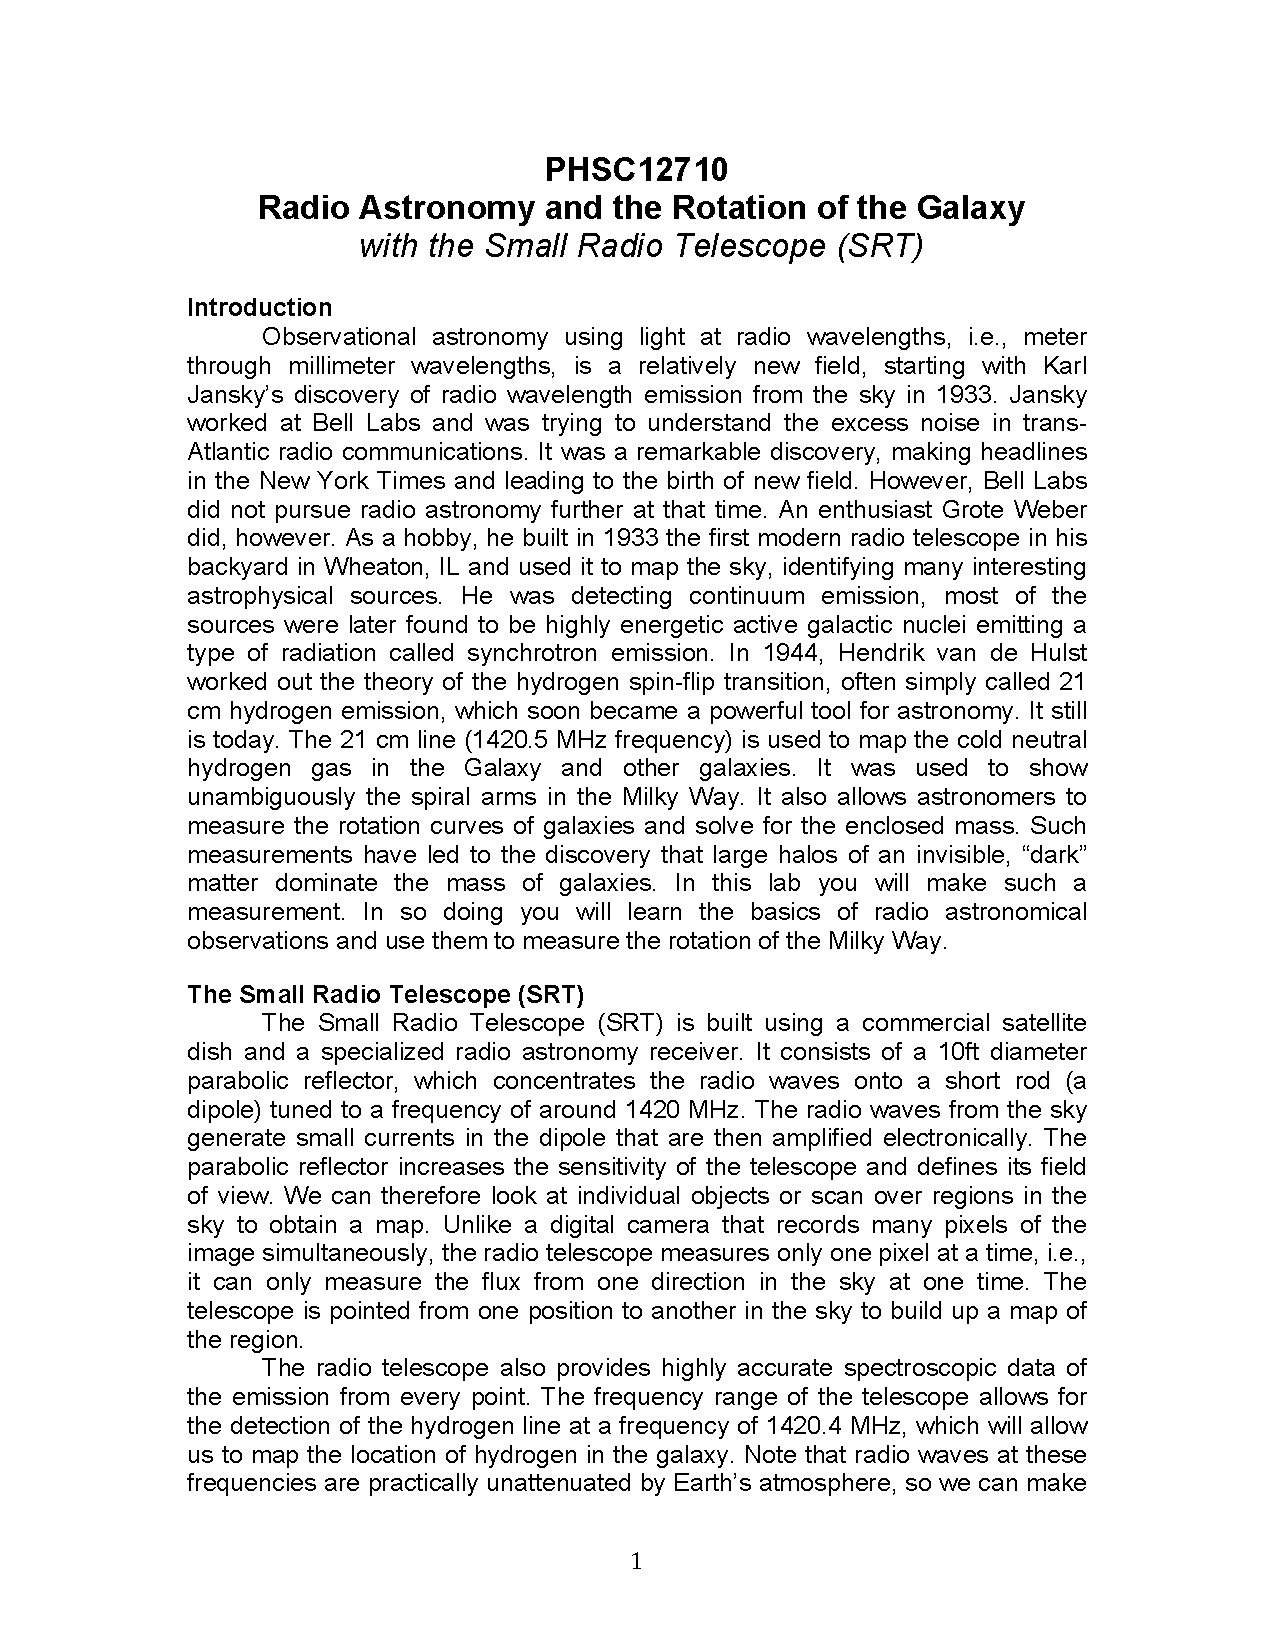
\includepdf[pages=-]{galaxy-rotation-srt/MilkyWayLab2018.pdf}

\appendix

\chapter{Analysis of Uncertainty}

A physical quantity consists of a value, unit, and uncertainty.
For example, ``$5 \pm 1\,$m'' means that the writer believes the true value of the quantity to most likely lie within 4 and 6 meters\footnote{The phrase ``most likely'' can mean different things depending on who is writing.
	If a physicist gives the value and does not given a further explanation, we can assume that they mean that the measurements are randomly distributed according to a normal distribution around the value given, with a standard deviation of the uncertainty given.
	So if one were to make the same measurement again, the author believes it has a 68\% chance of falling within the range given.
	Disciplines other than physics may intend the uncertainty to be 2 standard deviations.}.
Without knowing the uncertainty of a value, the quantity is next to useless.
For example, in our daily lives, we use an implied uncertainty.
If I say that we should meet at around 5:00 pm, and I arrive at 5:05 pm, you will probably consider that within the range that you would expect.
Perhaps your implied uncertainty is plus or minus 15 minutes.
On the other hand, if I said that we would meet at 5:07 pm, then if I arrive at 5:10 pm, you might be confused, since the implied uncertainty of that time value is more like 1 minute.

Scientists use the mathematics of probability and statistics, along with some intuition, to be precise and clear when talking about uncertainty, and it is vital to understand and report the uncertainty of quantitative results that we present.

\section{Types of measurement uncertainty}

For simplicity, we limit ourselves to the consideration of two types of uncertainty in this lab course, instrumental and random uncertainty.

\subsection{Instrumental uncertainties}

Every measuring instrument has an inherent uncertainty that is determined by the precision	
  of the instrument.
Usually this value is taken as a half of the smallest increment of the instrument's scale. For example, $0.5\:$mm is the precision of a standard metric ruler; $0.5\:$s is the precision of a watch, etc. For electronic digital displays, the equipment's manual often gives the instrument's resolution, which may be larger than that given by the rule above.

Instrumental uncertainties are the easiest ones to estimate, but they are not the only source of the uncertainty in your measured value.
You must be a skillful experimentalist to get rid of all other sources of uncertainty so that all that is left is instrumental uncertainty.

\subsection{Random uncertainties}

Very often when you measure the same physical quantity multiple times, you can get different results each time you measure it.
That happens because different uncontrollable factors affect your results randomly.
This type of uncertainty, random uncertainty, can be estimated only by repeating the same measurement several times.
For example if you measure the distance from a cannon to the place where the fired cannonball hits the ground, you could get different distances every time you repeat the same experiment.	
  
For example, say you took three measurements and obtained 55.7, 49.0, 52.5, 42.4, and 60.2 meters. We can quantify the variation in these measurements by finding their standard deviation using a calculator, spreadsheet, or the formula (assuming the data distributed according to a normal distribution)
\begin{equation}
 \sigma = \sqrt{\sum_{i=1}^{N} \frac{(x_i-\bar{x})^2}{N-1}} \, ,
\end{equation}
where $\{x_1, x_2, \dots, x_N\}$ are the measured values, $\bar{x}$ is the mean of those values, and $N$ is the number of measurements.
For our example, the resulting standard deviation is 6.8 meters. Generally we are interested not in the variation of the measurements themselves, but how uncertain we are of the average of the measurements. The uncertainty of this mean value is given, for a normal distribution, by the so-called ``standard deviation of the mean'', which can be found by dividing the standard deviation by the square root of the number of measurements,
\begin{equation}
\sigma_\textrm{mean} = \frac{\sigma}{\sqrt{N}} \, .
\end{equation}
So, in this example, the uncertainty of the mean is 3.0 meters. We can thus report the length as $52 \pm 3\:$m.

Note that if we take more measurements, the standard deviation of those measurements will not generally change, since the variability of our measurements shouldn't change over time. However, the standard deviation of the mean, and thus the uncertainty, will decrease.

\section{Propagation of uncertainty}

When we use an uncertain quantity in a calculation, the result is also uncertain. To determine by how much, we give some simple rules for basic calculations, and then a more general rule for use with any calculation which requires knowledge of calculus. Note that these rules are strictly valid only for values that are normally distributed, though for the purpose of this course, we will use these formulas regardless of the underlying distributions, unless otherwise stated, for simplicity.

If the measurements are completely independent of each other, then for quantities $a \pm \delta a$ and $b \pm \delta b$, we can use the following formulas:
\begin{equation}\label{unc:add}
\textrm{For } c = a + b \textrm{ (or for subtraction), } \delta c = \sqrt{(\delta a)^2 + (\delta b)^2}
\end{equation}

\begin{equation}\label{unc:mult}
\textrm{For } c = ab \textrm{ (or for division), } \frac{\delta c}{c} = \sqrt{\left(\frac{\delta a}{a}\right)^2 + \left(\frac{\delta b}{b}\right)^2}
\end{equation}

\begin{equation}\label{unc:exp}
\textrm{For } c = a^n,\, \frac{\delta c}{c} = n \frac{\delta a}{a}
\end{equation}

If you are familiar with calculus, you may want to use this general formula for the uncertainty $\delta f$ of a function $f$ of $N$ independent values $x_i$, each with uncertainty $\delta x_i$:
\begin{equation}\label{unc:general}
\delta f = \sqrt{ \sum_{i=1}^{N} \left(\frac{\partial f}{\partial x_i} \delta x_i\right)^2 } \, .
\end{equation}
Notice that Eqs.\ \ref{unc:add} through \ref{unc:exp} can be derived from Eq.\ \ref{unc:general} for those specific cases.

\subsubsection{What if there is no reported uncertainty?}

Sometimes you'll be calculating with numbers that have no uncertainty given.
In some cases, the number is exact.
For example, the circumference $C$ of a circle is given by $C = 2 \pi r$. Here, the coefficient, $2\pi$, is an exact quantity and you can treat its uncertainty as zero.
If you find a value that you think is uncertain, but the uncertainty is not given, a good rule of thumb is to assume that the uncertainty is half the right-most significant digit.
So if you are given a measured length of $1400\:$m, then you might assume that the uncertainty is $50\:$m.
This is an assumption, however, and should be described as such in your lab report.
For more examples, see Table~\ref{unc:tab:implied}.

\begin{table}
	\begin{center}
		\begin{tabular}{cc}
			\textbf{Expression} & \textbf{Implied uncertainty} \\
			12 & 0.5 \\
			12.0 & 0.05 \\
			120 & 5 \\
			120. & 0.5
		\end{tabular}
		\caption{Expression of numbers and their implied uncertainty.}\label{unc:tab:implied}
	\end{center}
\end{table}

\subsubsection{How many digits to report?}

After even a single calculation, a calculator will often give ten or more digits in an answer.
For example, if I travel $11.3 \pm 0.1\:$km in $350 \pm 10\:$s, then my average speed will be the distance divided by the duration. Entering this into my calculator, I get the resulting value ``\texttt{0.0322857142857143}''.
Perhaps it is obvious that my distance and duration measurements were not precise enough for all of those digits to be useful information.
We can use the propagated uncertainty to decide how many decimals to include.
Using the formulas above, I find that the uncertainty in the speed is given by my calculator as ``\texttt{9.65683578099600e-04}'', where the `\texttt{e}' stands for ``times ten to the''.
I definitely do not know my uncertainty to 14 decimal places.
For reporting uncertainties, it general suffices to use just the 1 or 2 left-most significant digits, unless you have a more sophisticated method of quantifying your uncertainties.
So here, I would round this to 1 significant digit, resulting in an uncertainty of $0.001\:$km/s.
Now I have a guide for how many digits to report in my value.
Any decimal places to the right of the one given in the uncertainty are distinctly unhelpful, so I report my average speed as ``$0.032 \pm 0.001\:$km/s''.
You may also see the equivalent, more succinct notation ``$0.032(1)\:$km/s''.

\section{Comparing two values}\label{unc:sec:comparing}

If we compare two quantities and want to find out how different they are from each other, we can use a measure we call a $t'$ value (pronounced ``tee prime''). This measure is not a standard statistical measure, but it is simple and its meaning is clear for us.

Operationally, for two quantities having the same unit, $a \pm \delta a$ and $b \pm \delta b$, the measure is defined as\footnote{Statistically, if $\delta a$ and $\delta b$ are uncorrelated, random uncertainties, then $t'$ represents how many standard deviations the difference $a - b$ is away from zero.}

\begin{equation}
%t' = \frac{\abs{a-b}}{\sqrt{(\delta a)^2 + (\delta b)^2}}
t' = \frac{\abs{a-b}}{\sqrt{(\delta a)^2 + (\delta b)^2}}
\end{equation}

If $t' \lesssim 1$, then the values are so close to each other that they are indistinguishable. It is either that they represent the same true value, or that the measurement should be improved to reduce the uncertainty.

If $1 \lesssim t' \lesssim 3$, then the result is inconclusive. One should improve the experiment to reduce the uncertainty.

If $t' \gtrsim 3$, then the true values are very probably different from each other.
%\begin{landscape}
\chapter{Rubrics}
	
	\freetabcaption{Rubric B: Ability to design and conduct an observational experiment \cite{etkina_scientific_2006}.}
	\begin{longtable}{>{\bfseries}p{0.02\textheight}|>{\bfseries\RaggedRight}p{0.25\textheight}|>{\RaggedRight}p{0.21\textheight}|>{\RaggedRight}p{0.21\textheight}|>{\RaggedRight}p{0.22\textheight}|>{\RaggedRight}p{0.22\textheight}}
		\toprule
		& Scientific Ability
		& Missing & Inadequate & Needs Improvement & Adequate \\ \midrule \endhead
		B1
		& Is able to identify the phenomenon to be investigated
		& No phenomenon is mentioned
		& The description of the phenomenon to be investigated is confusing, or it is not the phenomenon of interest.
		& \midsloppy The description of the phenomenon is vague or incomplete.
		& The phenomenon to be investigated is clearly stated. \\ \midrule
		B2
		& Is able to design a reliable experiment that investigates the phenomenon
		& The experiment does not investigate the phenomenon.
		& The experiment may not yield any interesting patterns.
		& Some important aspects of the phenomenon will not be observable.
		& The experiment might yield interesting patterns relevant to the investigation of the phenomenon. \\ \midrule
		B3
		& Is able to decide what physical quantities are to be measured and identify independent and dependent variables
		& The physical quantities are irrelevant.
		& Only some of physical quantities are relevant.
		& The physical quantities are relevant. However, independent and dependent variables are not identified.
		& The physical quantities are relevant and independent and dependent variables are identified. \\ \midrule
		B4
		& Is able to describe how to use available equipment to make measurements
		& At least one of the chosen measurements cannot be made with the available equipment.
		& All chosen measurements can be made, but no details are given about how it is done.
		& All chosen measurements can be made, but the details of how it is done are vague or incomplete.
		& All chosen measurements can be made and all details of how it is done are clearly provided. \\ \midrule
		B5
		& Is able to describe what is observed without trying to explain, both in words and by means of a picture of the experimental setup.
		& No description is mentioned.
		& A description is incomplete. No labeled sketch is present. Or, observations are adjusted to fit expectations.
		& A description is complete, but mixed up with explanations or pattern. Or the sketch is present but is difficult to understand.
		& Clearly describes what happens in the experiments both verbally and with a sketch. Provides other representations when necessary (tables and graphs). \\ \midrule
		B6
		& Is able to identify the shortcomings in an experiment and suggest improvements
		& No attempt is made to identify any shortcomings of the experiment.
		& The shortcomings are described vaguely and no suggestions for improvement are made.
		& Not all aspects of the design are considered in terms of shortcomings or improvements.
		& All major shortcomings of the experiment are identified and reasonable suggestions for improvement are made. \\ \midrule
		B7
		& Is able to identify a pattern in the data
		& No attempt is made to search for a pattern.
		& The pattern described is irrelevant or inconsistent with the data.
		& The pattern has minor errors or omissions. Terms like ``proportional'' used without clarity, e.g.\ is the proportionality linear, quadratic, etc.
		& The pattern represents the relevant trend in the data. When possible, the trend is described in words. \\ \midrule
		B8
		& Is able to represent a pattern mathematically (if applicable)
		& No attempt is made to represent a pattern mathematically.
		& The mathematical expression does not represent the trend.
		& No analysis of how well the expression agrees with the data is included, or some features of the pattern are missing.
		& The expression represents the trend completely and an analysis of how well it agrees with the data is included. \\ \midrule
		B9
		& Is able to devise an explanation for an observed pattern
		& No attempt is made to explain the observed pattern.
		& An explanation is vague, not testable, or contradicts the pattern.
		& An explanation contradicts previous knowledge or the reasoning is flawed.
		& A reasonable explanation is made. It is testable and it explains the observed pattern. \\
		\bottomrule
	\end{longtable}

	
%\end{table}

\end{landscape}
% This format is not a formal report, but simply answering questions, including figures, and demonstrating scientific abilities.
\chapter{Lab Report Format}\label{cha:lab-report-format}

%TODO Make firm page limit? 5 pages + figures and tables?

%In a general sense, the labs should demonstrate the rubric rows listed in the lab write-up and provide answers to every lab question asked.

\section{General}

\begin{itemize}
	\item The report should be typed for ease of reading. Text should be double-spaced, and the page margins (including headers and footers) should be approximately $2.5\:$cm, for ease of marking by the grader. Each page should be numbered.
	
	\item The first page should include the title of the lab; lab section day, time, and number; and the names of the members of your lab team.
	
%	\item If the rubric row refers to a particular part of your lab report, clearly label that part of the report with that rubric row. For example, you should label the section where you demonstrate uncertainty propagation with ``G2'' if that rubric row is being assessed in that lab.
\end{itemize}

\section{Organizing the report}

%If the lab is clearly framed as an observational, testing, or application experiment, you can follow the corresponding rubric for the elements to include in the report (see, respectively, Rubrics B, C, and D in Appendix~\ref{cha:rubrics}).

The report should follow the sequence of the report checklist. Answers to questions and inclusion of tables and figures should appear in the order they are referenced in the manual. In general, include the following:

	\begin{itemize}
%		\item Any procedure that you performed that is different from what is described in the lab manual.
		
%		\item Any data that you've collected: tables, figures, measured values, sketches. Whenever possible, include an estimate of the uncertainty of measured values.
		
		\item For any calculations that you perform using your data, and the final results of your calculation, you must show your work in order to demonstrate to the grader that you have actually done it. Even if you're just plugging numbers into an equation, you should write down the equation and all the values that go into it. This includes calculating uncertainty and propagation of uncertainty.
		
		\item If you are using software to perform a calculation, you should explicitly record what you've done. For example, ``Using Excel we fit a straight line to the velocity vs. time graph. The resulting equation is $v = (0.92\:\mathrm{m/s^2}) t + 0.2\:\mathrm{m/s}$.''
		
		\item Answers to any questions that appear in the lab handout. Each answer requires providing justification for your answer.
		
%		\item At the end of each experiment, you should discuss the findings and reflect deeply on the quality and importance of the findings%
		% (Rubric Row F2)
%		. This can be both in the frame of a scientist conducting the experiment (``What did the experiment tell us about the world?'') and in the frame of a student (``What skills or mindsets did I learn?'').
	\end{itemize}

\section{Graphs, Tables, and Figures}

Any graph, table, or figure (a figure is any graphic, for example a sketch) should include a caption describing what it is about and what features are important, or any helpful orientation to it. The reader should be able to understand the basics of what a graph, table, or figure is saying and why it is important without referring to the text. For more examples, see any such element in this lab manual.

Each of these elements has some particular conventions.

\subsection{Tables}

A table is a way to represent tabular data in a quantitative, precise form. Each column in the table should have a heading that describes the quantity name and the unit abbreviation in parentheses. For example, if you are reporting distance in parsecs, then the column heading should be something like ``distance (pc)''. This way, when reporting the distance itself in the column, you do not need to list the unit with every number.

\subsection{Graphs}

A graph is a visual way of representing data. It is helpful for communicating a visual summary of the data and any patterns that are found.

The following are necessary elements of a graph of two-dimensional data (for example, distance vs. time, or current vs. voltage) presented in a scatter plot.

\begin{itemize}
	\item \textbf{Proper axes.} The conventional way of reading a graph is to see how the variable on the vertical axis changes when the variable on the horizontal axis changes. If there are independent and dependent variables, then the independent variable should be along the horizontal axis.
	
	\item \textbf{Axis labels.} The axes should each be labeled with the quantity name and the unit abbreviation in parentheses. For example, if you are plotting distance in parsecs, then the axis label should be something like ``distance (pc)''.
	
	\item \textbf{Uncertainty bars.} If any quantities have an uncertainty, then these should be represented with so-called ``error bars'', along both axes if present. If the uncertainties are smaller than the symbol used for the data points, then this should be explained in the caption.

\end{itemize}

%\chapter{Manual: PASCO Cavendish Balance}\label{cha:pasco-cavendish}

On the following pages is the manual for the PASCO Cavendish Balance.

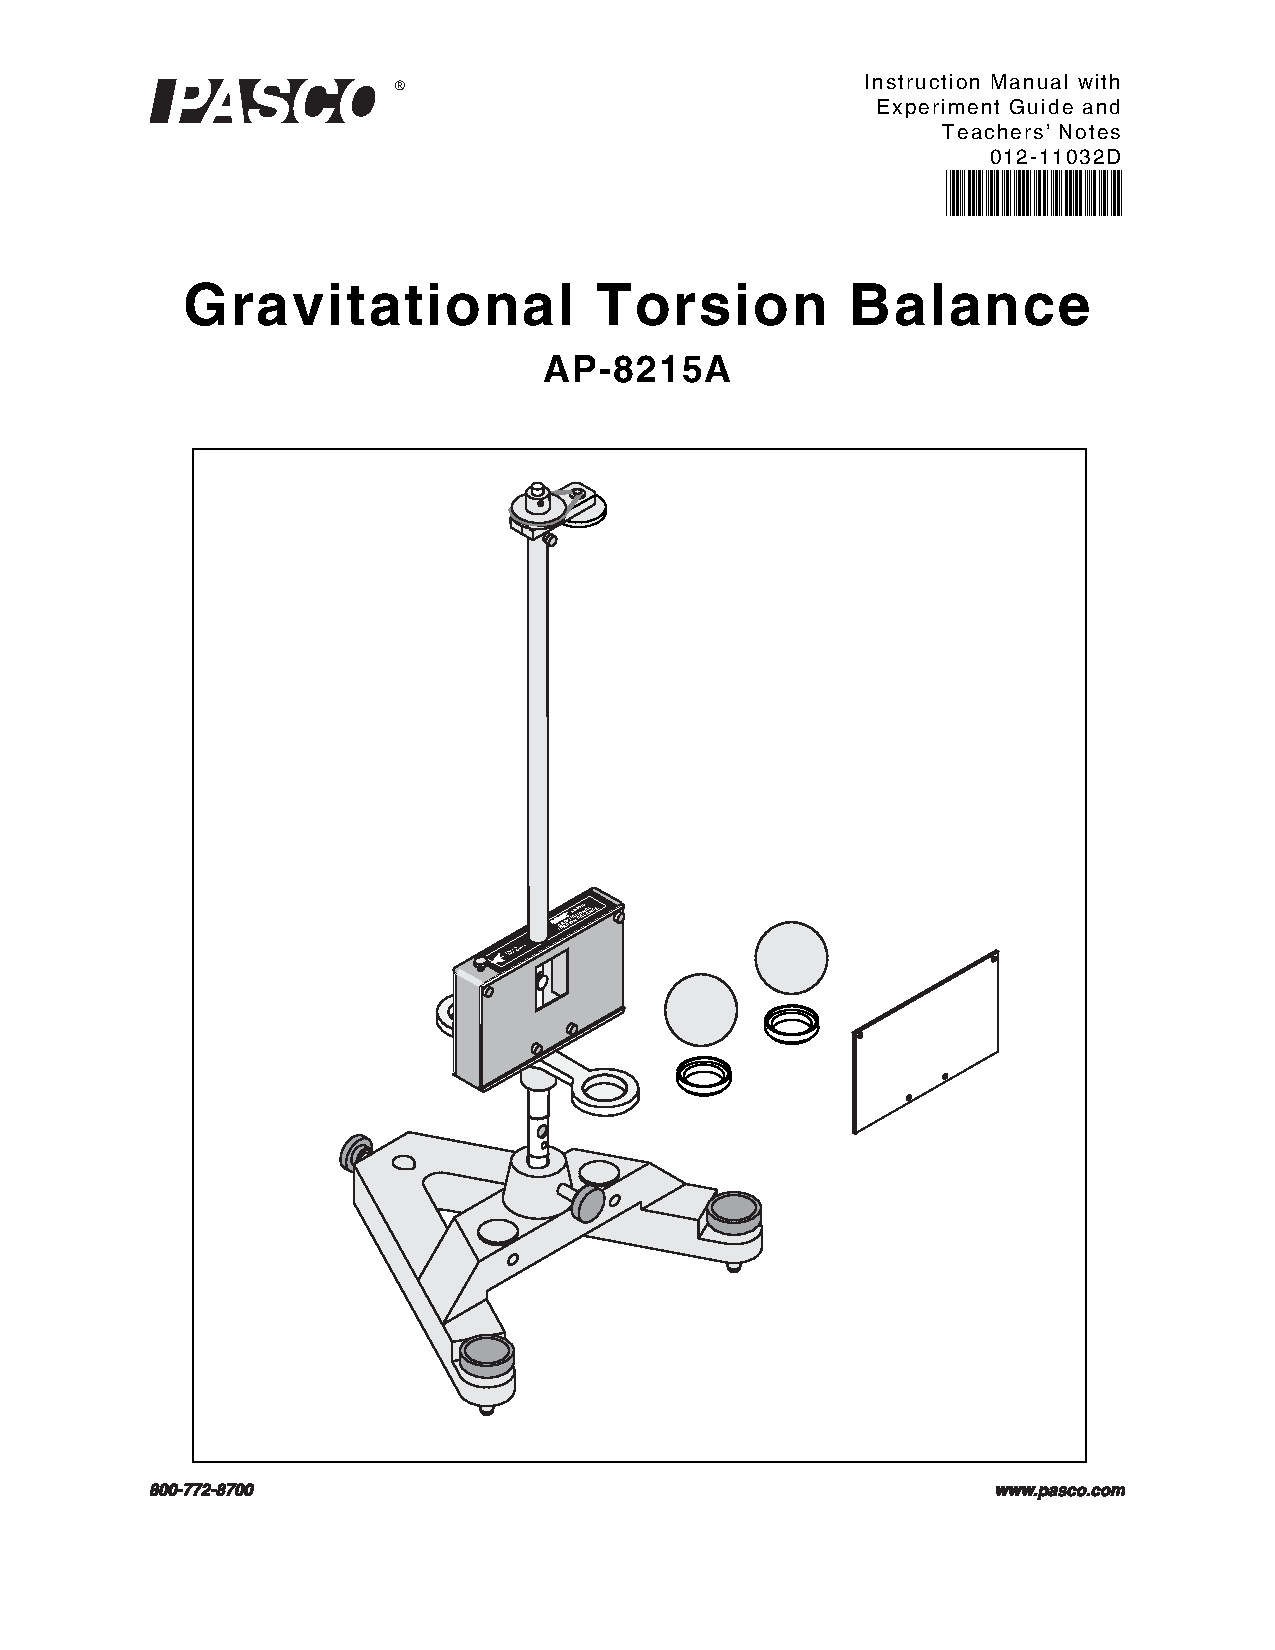
\includepdf[pages={1,3-8,16}]{pasco-cavendish/Gravitational-Torsion-Balance-Manual-AP-8215A.pdf}

% \bibliography{references,MyLibrary}
% \bibliographystyle{plain}
\printbibliography

\end{document}
